% kompiliert mit XeLaTeX
\documentclass[
11pt, % font size
parskip=half, % space between paragraphs instead of indentation
digital, % digital or print
oneside, % oneside / twoside
%	openright, % openright for title page and subsequent chapters on right pages in twosided layout
]{bsc}

\usepackage {xltxtra}
\usepackage{microtype}
% Package für Bilder
\usepackage{graphicx}
\usepackage{enumitem}

\title{Understanding}
\author{Max SImon}
\date{August 21, 2017}

% Mathe
\usepackage{amsmath, amssymb, booktabs, hyperref, subcaption, siunitx}

\bibliography{Paper}

% Code
\usepackage{listings}

\newcommand{\diff}{\text{d}}
\newcommand{\pip}{PI(4,5)P$_2$}
\newcommand{\acid}[2]{#1$^{#2}$}


\newcommand{\gromacs}{GROMACS}
\newcommand{\martini}{MARTINI}
\newcommand{\charmm}{CHARMM36}
\newcommand{\conan}{CONAN}

\newcommand{\pope}{POPE}
\newcommand{\popc}{POPC}
\newcommand{\forceunit}{\si{\pico\newton}}

% MyFig: \myFig[width]{source}{label}{figure title}{text}
\newcommand{\nicecaption}[2]{\caption[#1]{\small{\textbf{#1}\\#2}}}


%\includeonly{results}

\begin{document}
% abstract english
%\chapter*{Abstract}
Focal adhesion kinase (FAK) is a tyrosine kinase associated to focal adhesions with a downstream effect on cell migration and other biological functions. The phospholipid \pip{} is known as a moderator for FAK activation. \pip{} induces clustering of FAK molecules, but the impact of clustering on the protein conformation of FAK is still not understood. Since an overexpression of FAK is associated with invasive tumours, insights into the clustering process could give rise to new cancer treatments.\\
In previous studies, coarse-grained MD simulations led to an unnatural falling of FAK on the membrane. During the course of this project, we were able to rule out an underestimation of the binding strength of FAK to \pip{} as the cause using umbrella simulations. Because the exact reason for FAK falling could not be identified, we introduced a stabilising force acting on the FERM domain of FAK. With this approach, we obtain reasonable results for FAK bound to \pip{} as well as for multiple FAK interactions. Our observations indicate that FAK arranges into chain-like clusters. However, we do not observe FAK activation upon clustering within the time-scale of our simulations.
\newpage
\leavevmode\thispagestyle{empty}\newpage
\chapter*{Zusammenfassung}
\begin{german}
	FAK ist eine Tyrosinkinase, die vermehrt in Fokalen Adhäsionen zu finden ist und regulierende Einflüsse auf Zellmigration und andere biologische Funktionen hat. Als Moderator der Aktivierung von FAK tritt das Phospholipid \pip{} auf. \pip{} induziert die Bildung von FAK-Clustern. Allerdings ist der Einfluss der Clusterbildung auf die Konformation von FAK noch nicht vollständig verstanden. Da in invasiven Tumoren häufig eine überdurchschnittlich hohe Konzentration von FAK zu finden ist, könnte ein tieferes Verständnis der Clusterbildung ein wichtiger Schritt auf dem Weg hin zu neuartigen Krebstherapien sein.\\
	In vorangegangen Untersuchungen führte die Verwendung von grobaufgelösten MD Simulationen zu einem unnatürlichen Umfallen von FAK auf die Seite. Im Verlauf dieses Projektes konnten wir mit Hilfe von Umbrella Sampling die Unterschätzung der Energie der Hauptbindungsstelle von FAK zu \pip{} als Ursache ausschließen. Da der tatsächliche Grund des Umfallens nicht identifiziert werden konnte, führten wir eine stabilisierende Kraft auf die FERM Domäne von FAK ein. Mit diesem Ansatz können wir plausible Ergebnisse für FAK gebunden an \pip{} und Interaktionen zwischen mehreren FAK beobachten. Unsere Beobachtungen deuten darauf hin, dass FAK-Moleküle zu einer kettenartigen Strukturbildung tendieren. Allerdings kann in derartigen Strukturen keine signifikante Aktivierung von FAK beobachtet werden.
\end{german}
\newpage

%	
%	
% chapter introduction
\chapter{Introduction}
Focal adhesions (FA) are macromolecular protein complexes which act as a connection hub between the cell, especially the cytoskeleton, and the extracellular matrix (ECM). They enable the cell to exert tension forces, but can also transduce mechanical stimuli from the ECM to the inside of the cell and integrate this information. One important protein associated to FAs is the focal adhesion kinase (FAK). FAK occurs in several signalling pathways and is a key player in integrating extracellular stimuli. It is of large interest not least because often an overexpression of FAK can be found in cancer cells, and understanding the activation processes and dynamics of FAK could give rise to new cancer treatments \autocite{cancerFAK}.
\section{Structure}
FAK consists of four domains: (i) a FERM (4.1 protein, ezrin, radixin and moesin) domain at the N-terminus, (ii) a tyrosine kinase, (iii) a proline-rich region and (iv) a focal adhesion targeting (FAT) domain at the C-terminus (\autoref{intro:fak}).\\
FERM is a common protein domain which links proteins to membranes by binding to various phospholipids \autocite{fermdomain} and consists of three subdomains: F1, F2 and F3. In the F2 subdomain, a basic patch ($^{216}$KAKTLRK$^{222}$) can be found, which is a prominent binding site for phosphatidylinositol-4,5-bisphosphate (\pip).\\
The kinase consists of a C-lobe, an activation loop and an N-lobe. Catalytic activity of the kinase is mainly regulated by the phosphorylation of \acid{Y}{576}{} and \acid{Y}{577}, which are located in the activation loop \autocite{tyrosinePhosphor}. The kinase also provides binding sites for \pip{}. One is located next to the basic patch of the FERM domain, but others (namely \acid{R}{508}, \acid{R}{514}, \acid{K}{515}, \acid{K}{621} and \acid{K}{627}) can be found on the side of the kinase \autocites{pap002}{pap002Exp}.\\
The FERM domain and the kinase are connected by a linker region. In contrast to other kinase domains, the main autophosphorylation site of FAK, \acid{Y}{397}, can be found in this region and not in the kinase itself \autocite{pap001}.\\ %TODO: better cite
The FAT domain is linked to the kinase by a flexible proline-rich region. FAT links to FAs by interacting with talin and paxillin which are integrin-associated proteins \autocite{fatdomain}.
%
%
%
\begin{figure}
	\centering
	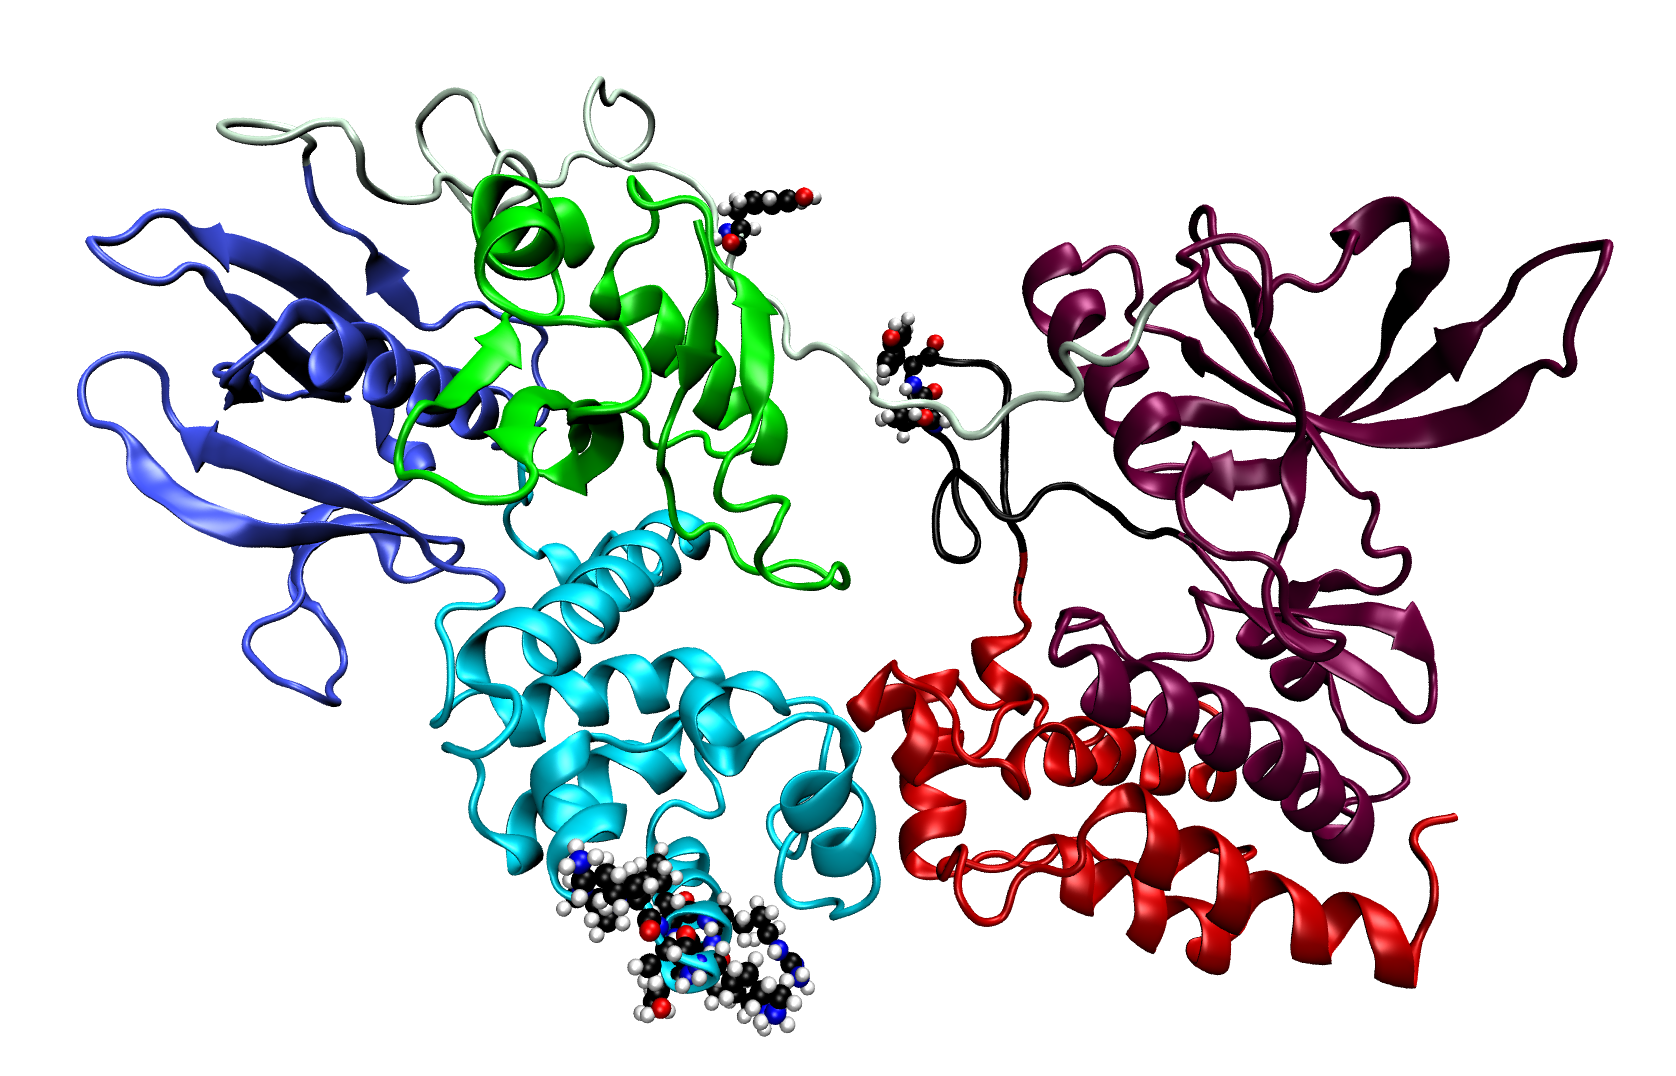
\includegraphics[height=6cm]{figures/introduction/fak}
	\nicecaption{Structure of FAK}{The FERM domain consisting of F1 (green), F2 (iceblue) and F3 (blue) connected via the linker to the kinase consisting of N-lobe (violet), activation loop (black) and C-lobe (red). The basic patch (F2), \acid{Y}{397} (linker) and \acid{Y}{567}, \acid{Y}{577} (activation loop) are shown in atomistic representation.}
	\label{intro:fak}
\end{figure}
%
%
%
\section{\pip{} binding and activation}
It is known that FAK triggers several stimuli with a downstream effect on e.g. cell migration \autocite{cellMigration}. However, the focus in this thesis is on the interactions with \pip{}. Therefore, only the different binding sites of FAK for \pip{} and their impacts on FAK activation are discussed in the following.\\
\\
In the autoinhibited conformation, the FERM domain shields the active site of the kinase. An activation of FAK therefore requires the dissociation of the FERM and the kinase \autocite{structFAK}.\\
\pip{} is a phospholipid which is locally generated in FAs due to integrin signalling \autocite{pip2LocalGeneration}. Its charge depends strongly on the pH, but at physological conditions a net charge of -4 is the preferred state. However, in presence of basic amino acids (Arg, Lys), the deprotonated state gets promoted, resulting in a net charge of -5 \autocite{pip2_minus5}. The electrostatic binding of \pip{} to the basic patch in the F2 subdomain results in allosteric changes, which also influence the interface between the F1 subdomain and the N-lobe. Moreover, the linker region gets less strongly bound, which promotes autophosphorylation of \acid{Y}{397}. However, the \pip{} binding alone has no effect on the catalytic activity, which suggests that the FERM domain is still associated to the kinase \autocites{pap001}{pap003}. For activation, an additional stimulus, either biochemical or mechanical, is needed.\\
\\
If \acid{Y}{397} is phosphorylated, it becomes a suitable binding site for SH2 or SH3, which are subdomains of proteins of Src family tyrosine kinases. Due to the conformational changes induced by \pip{}, this kinase has access to \acid{Y}{576} and \acid{Y}{577}. As said, the phosphorylation of these residues makes FAK fully active, resulting in dissociation of the FERM domain and the kinase \autocite{pap001}.\\
\\
Mechanical forces can lead to dissociation of the FERM domain from the kinase as well. Forces acting on the FAT domain are transduced to the interface of the FERM domain and the kinase because the linker is connected to the kinase, while the FERM domain is anchored onto a \pip{} containing membrane. These forces can lead to activation of FAK. In that way, it is acting as a mechanical sensor \autocite{pap004}.\\
\\
The binding sites on the side of the kinase were identified by computer simulations \autocite{pap002} and have been confirmed recently in experiments \autocite{pap002Exp}. The findings from \textcite{pap002Exp} show that these residues are required for catalytic activity of the kinase, and that they bind to phospholipids \textit{in vivo}. However, since the catalytic activity is not regulated by \pip{}, this binding was hypothesized to act as a stabilisation of the active state only \autocite{pap002Exp}.
\section{Dimerization, clustering and autophosphorylation}
\label{intro:clustering}
Autophosphorylation of \acid{Y}{397} is an important event in FAK activation. It has been shown that this happens in intact cells \textit{in trans}, for which a self-association of FAK is required \autocite{transAuto}.\\
\\
The FERM domain induces a dimerization of FAK, as it does in other proteins containing a FERM domain as well. % TODO: in vivo, in vitro?
The interaction emerges around \acid{W}{266} in the connected FERM domains and is stabilised by an interaction of the FAT domain with the basic patch of the other FERM domain, respectively. The presence of \acid{W}{266} is also required for autophosphorylation of FAK.\\
\pip{} is not needed for the dimerization of the FERM domains. However, an enriched FAK concentration is needed to observe FAK dimers in cells, which is the case at FAs. It is still unclear how the dimer is stabilised at membranes, where the basic patch is also required for ligand binding \autocite{fakdimers}.\\
It has been shown that \textit{in trans} autophosphorylation of FAK is promoted by dimerization \autocite{dimersVsClusters}.\\
\\
Albeit \pip{} is not required for dimerization, it induces clustering of several FAK molecules on the membrane \textit{in vitro} \autocite{pap001}. Because dimers support autophosphorylation of FAK, it is not surprising that the same effect is observed in clusters. However, these clusters can trigger additional biochemical stimuli \autocite{dimersVsClusters} and may play an important role in the scaffolding function of FAK for FAs \autocite{pap001}.

%
%
% chapter motivation
\label{motivation}
As described in \autoref{intro:clustering} the process of FAK clustering and its effect upon activation, especially on an atomistic scale, are still not understood and part of current research. In this thesis the results of MD simulations with the Martini force field (see \autoref{subsub:coarsegraining}) are presented, which address the clustering process of FAK molecules. In this context Martini is a necessary simplification due to the large number of particles in systems containing sever FAK molecules.\\
\\
However previous work in the group \autocite{sara} obtained difficulties in the use of Martini for simulations of FAK on a \pip{} containing membrane. In some simulations equivalent to setup 3 (see \autoref{setup:setup3}) except for an external force the protein rapidly changed its inclination to the membrane. In the following part this shall be characterised by the angle $\beta$ between the z-axis and the vector connecting F1 and F2, $\vec{d}_F$.
\begin{equation}
\cos\left(\beta\right) = \frac{\vec{d}_{F, z}}{d_F},\quad d_F = \left|\vec{d}_F\right|
\end{equation}
\textcite{sara} simulated five different copies for $10\,\si{\micro\second}$ each. The resulting distributions of the angle can be seen in \autoref{motiv:sarascurves}. Exemplary the red line shows a mean value of $90\,\si{\deg}$, which is what meant with a falling of FAK in the following part. The angle changed in less than XXX and stayed constant for the remaining simulation time.\\
There are several reasons why this is rather an artefact of the Martini force field than a possible binding pose of FAK to the membrane as suggested by \textcite{pap002}. The first one is, that FAK falls to both extensive sites, which means that the key residues for an interaction of the extensive site of the kinase with the membrane proposed by \textcite{pap002} are located on top of the FAK and not on the side of the membrane. Indeed contact analysis showed, that virtually all residues on the surface (in both, FERM domain and kinase) were interacting with the membrane. Another one is, that this behaviour was not observed in equivalent all atom simulations in C36 ($1.5\,\si{\micro\second}$ in total). Here only two maxima were observed around $8\,\si{\deg}$ and around $20\,\si{\deg}$, the largest observed angle was $40\,\si{\deg}$.\\
\\
In the course of this project several efforts were made to understand the cause of this falling, e. g. to review the binding of the basic patch in Martini, which is presented in \autoref{results:umbrella}. However the reason could not have proven beyond doubt. In order to still perform reasonable simulations of multiple FAK an external force was applied to each FAK molecule. This is called stabilizing force in the following parts.\\
The force is acting onto F1 and F2 parallel to the z-axis and is proportional to the deviation of their z-distance $\Delta z$ from a reference distance $z_0$. An illustration of the force can be found in \autoref{motiv:forceillustr}. For the determination of $z_0$ only the green and the blue distribution from \autoref{motiv:sarascurves} were considered, because the large angles observed in the other distributions have not been observed in C36 simulations. The mean value of $\vec{d}_{F, z}$ for these two distributions is $2.228\,\si{\nano\metre}$, which was therefore set as $z_0$. %TODO: get force constant out of distribution
\textit{@Csaba: sorry, but how did we get this force constant of 1000 out of the distributions?}\\
\\
%
%
%
\begin{figure}
	\subcaptionbox{\label{motiv:sarascurves}}[0.49\textwidth]{
		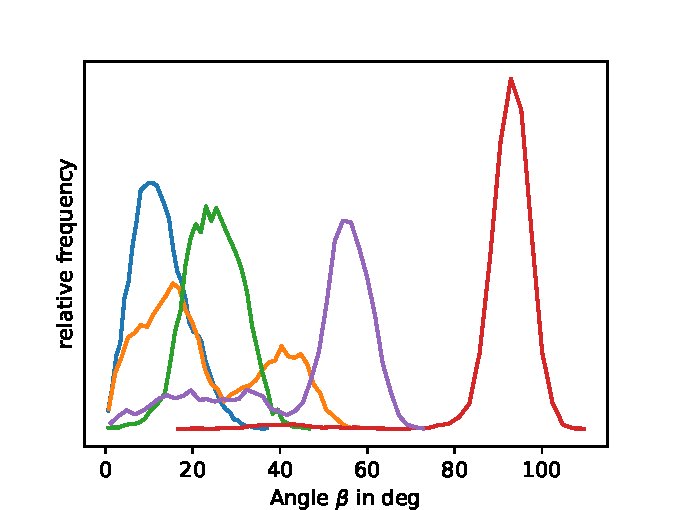
\includegraphics[height=5cm]{figures/introduction/sara_angles}
	}\hfill%
	\subcaptionbox{\label{motiv:forceillustr}}[0.49\textwidth]{
		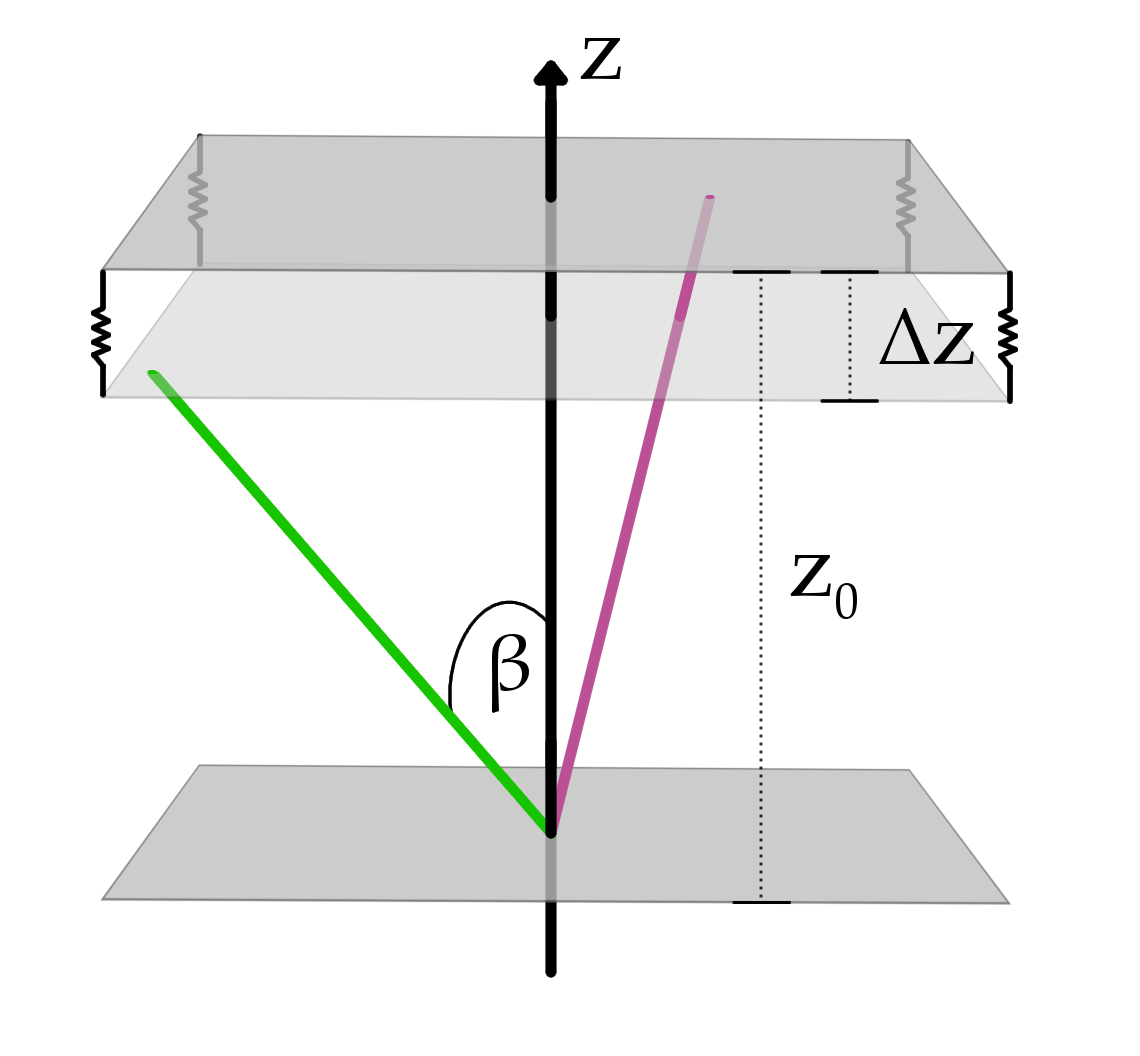
\includegraphics[height=5cm]{figures/introduction/forceapproach}
	}%
	\nicecaption{Inclination angle of FAK}{(\subref{motiv:sarascurves}): Distributions of $\beta$ obtained by \textcite{sara}. (\subref{motiv:forceillustr}): Illustration of the applied force.}
\end{figure}
%
%
%
In the following two chapters the used methods, i.e. MD simulation, are explained and the used setups introduced. Afterwards the obtained results are presented. For this purpose FAK in solution and FAK bound to \pip{} are analysed and compared to known information from experiments or other simulations. Also the impacts of the stabilizing force onto the simulations are commented. At last the focus is set on interactions between multiple FAK molecules.


%
%
% chapter methods
\section{Methods}
The present thesis is meant to give an insight into dynamics and characteristics of FAK-FAK interactions as well as interactions with a \pip{} containing membrane obtained from MD simulations. For this purpose the Martini force field and C36 were used.\\
All simulations were made with starting configurations adapted from previous work in the group (C36 forcefield: \textcite{pap003}, Martini forcefield: \textcite{SARA}). Only a FERM-kinase fragment without the FAT domain (residues 35 to 686, PDB 2J0J \autocite{structFAK}) was used. As simulation options the recommended values were used and can be found IN THE APPENDIX. All simulations have been done at a temperature of 300$\si{\kelvin}$.\\
As explained in \autoref{subsub:coarsegraining} proteins have to be stabilized in Martini with elastic networks. This was set up by \textcite{SARA} to act only inside domains with a force constant of 830 $\si{\kilo\joule\mole^{-1}\nano\meter^{-2}}$. Therefore the interface between FERM domain and kinase is not affected and the linker is still flexible.
\subsection{Free energy of \pip{} binding}
In the first part of this thesis the free energy landscape of the \pip{} binding to the basic patch was retrieved for C36, Martini and Martini with PW using umbrella sampling.\\
For simplicity only a part of the F2 subdomain was used (residues 107 to 219). The F2 was placed above a \pip{} embedded into a phosphatidylethanolamine (\pope{}) membrane (see PICTURE). The whole system was transferred to a Martini structure with a provided transformation tool \autocite{backwardpy} and the elastic network was applied.\\
After a short equilibration the protein was pulled slowly away from the membrane using a distance pull between the COM of the protein and the COM of the \pip{}. This simulation was used to retrieve starting conformations for the umbrella windows (between 90 and 120, dependent on the resulting sampling). Afterwards each umbrella window was equilibrated for 0.5$\si{\nano\second}$ and then simulated for 6$\si{\nano\second}$ (10$\si{\nano\second}$ for Martini and Martini with PW). For each forcefield the pulling and umbrella sampling was done five times to estimate the statistical error.\\
The presented results are based on a total simulation time of 6.33$\si{\micro\second}$ for Martini, 5.64$\si{\micro\second}$ for Martini with PW and 3.88$\si{\micro\second}$ for C36. % C36: 1=180, 4.2=135, 5=102, 5.2=102, 6=127, Mart: 1=134, 2=126, 3=130, 4=113, 5=130, MartPol: alle=113
\subsection{Binding pose on membrane}
Reasons, why Saras can not be.
All atom and Polarizable water.

%
%
% chapter setup
\chapter{Setup}
\section{Protein structure}
All simulations have been done with starting configurations adapted from previous work in the group (C36 forcefield: \textcite{pap003}, \martini{} forcefield: \textcite{sara}). These configurations contain only a FERM-kinase fragment without the FAT domain and its linker (only residues 35 to 686, PDB 2J0J \autocite{structFAK}).\\
As explained in \autoref{subsub:coarsegraining} the secondary structure of proteins have to be stabilized in \martini{} using elastic networks. This was set up by \textcite{sara} to act only between backbone beads of the same domain which are within a cut-off radius of $1\,\si{\nano\metre}$. Therefore, the interface between FERM domain and kinase is not affected and the linker is still flexible. The force constant is 830 $\si{\kilo\joule\mole^{-1}\nano\meter^{-2}}$. 
\section{Setup 1 - FAK in solution}
\label{setup:setup1}
Setup 1 refers to a \martini{} simulation of a single FAK molecule in waterbox. NaCl ions were added to neutralize the charge.\\
After a short equilibration the system was simulated for $20\,\si{\micro\second}$ at a temperature of $300\,\si{\kelvin}$. We used the default parameters of the \martini{} forcefield as input parameters.
%
%
%
\begin{figure}[h]
	\centering
	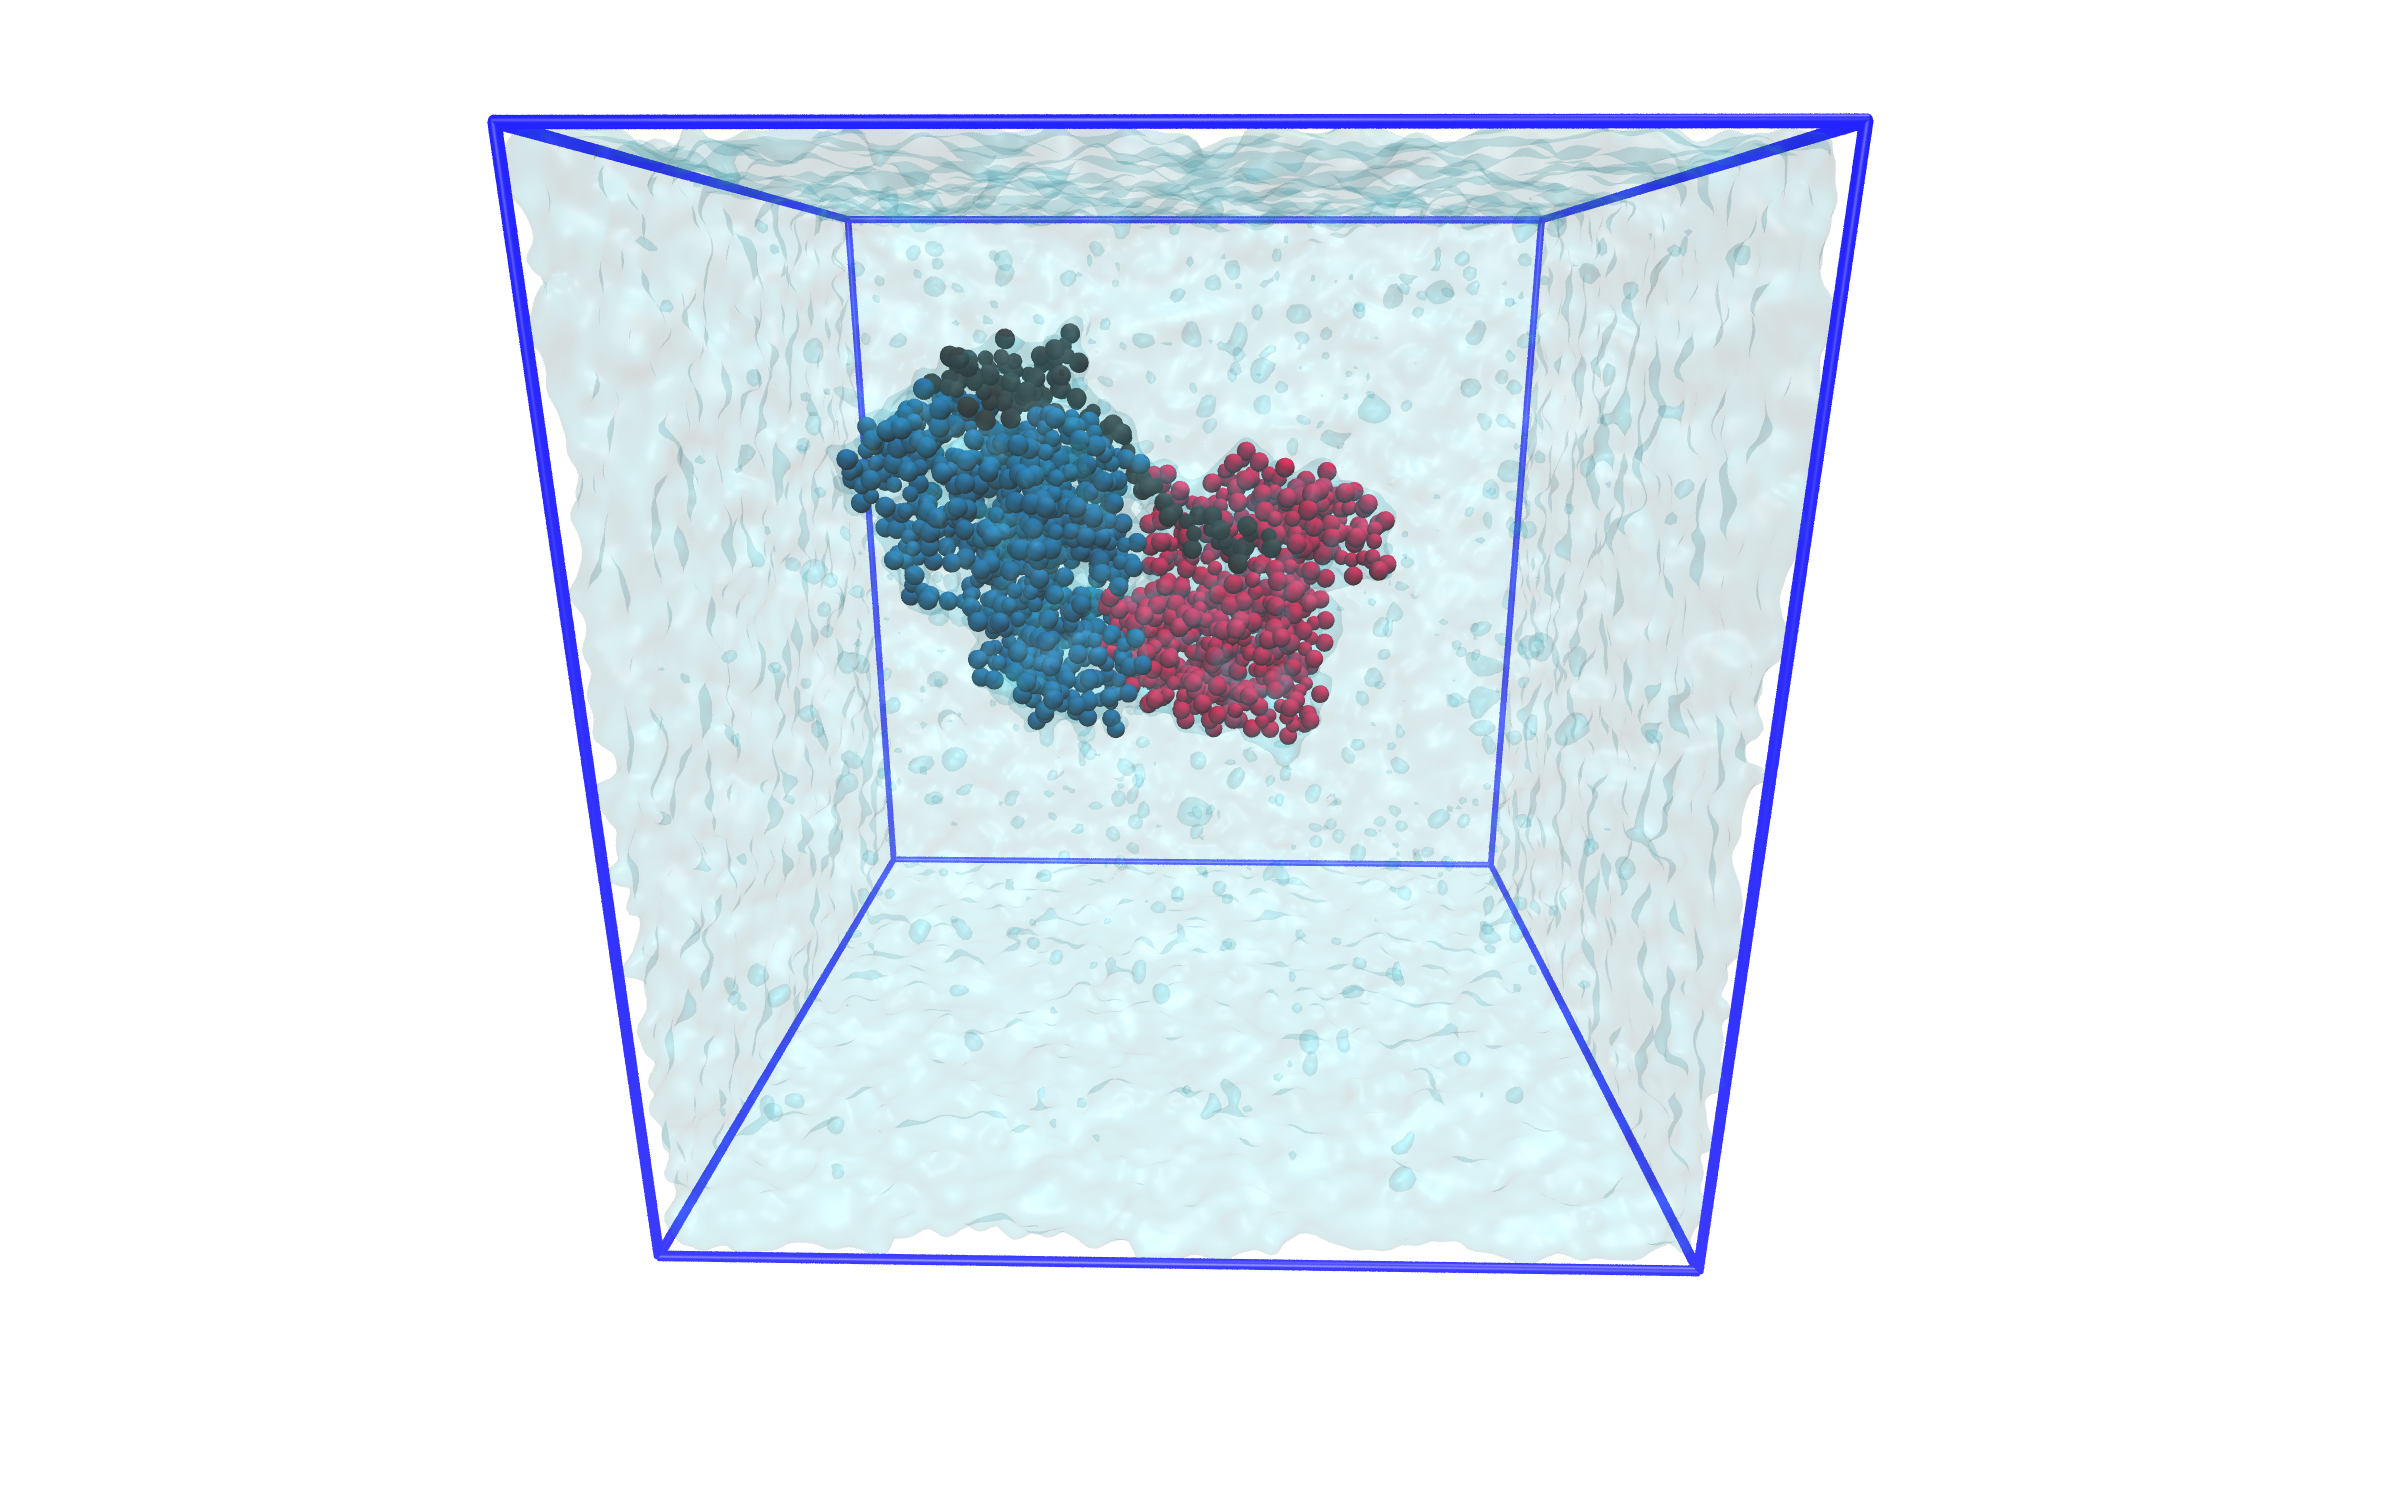
\includegraphics[height=6cm]{figures/setup/setup_free}
	\nicecaption{Setup 1 - FAK in solution}{The \martini{} structure of setup 1. The simulation box contains one FAK molecule (1486 beads) in water (~50 000 beads) with ions (23 sodium beads and 20 chlorine beads). The box dimensions are $18.8\,\si{\nano\metre}$ x $18.8\,\si{\nano\metre}$ x $18.8\,\si{\nano\metre}$}
	\label{setup:setup1_pic}
\end{figure}
%
%
%
\section{Setup 2 - Free energy of basic patch}
\label{setup:setup2}
For this setup only a part of F2 (residues 107 to 219, referred as F2 lobe in the following) was used. The lobe contains the basic patch and has a net charge of -5. Therefore no additional ions were needed.\\
We placed the lobe as a \charmm{} structure above a single \pip{} embedded into a phosphatidylethanolamine (\pope{}) membrane (see \autoref{tobeadded}). After a short equilibration, the F2 lobe was pulled slowly away from the membrane using a distance pull between the COM of the lobe and the COM of \pip{}. From this simulation, we retrieved starting conformations for the umbrella window. The number of umbrella windows was chosen accordingly to the sampling (between 90 and 120 windows). Each window was shortly equilibrated and afterwards simulated for $6\,\si{\nano\second}$.  From the trajectories of the umbrella windows the free energy profile was calculated using \gromacs{} WHAM implementation \autocite{gromacsWHAM}. The pulling and umbrella sampling was done five times to estimate the statistical error.\\
The starting configurations was transferred to a \martini{} structure (with both, standard water model and PW) with provided transformation tools \autocite{backward.py}. Afterwards the elastic network was applied. Analogously to the simulation in \charmm{}, we retrieved starting configurations for the umbrella windows and simulated them for five independent copies. The simulation time for one umbrella window was increased to $10\,\si{\nano\second}$.\\
The presented results are based on a total simulation time of $3.88\,\si{\micro\second}$ for C36, $6.33\,\si{\micro\second}$ for \martini{}, $5.64\,\si{\micro\second}$ for \martini{} with PW. The temperature in the simulations was kept at $300\,\si{\kelvin}$. For all three force fields the default parameters were used.
% C36: 1=180, 4.2=135, 5=102, 5.2=102, 6=127, Mart: 1=134, 2=126, 3=130, 4=113, 5=130, MartPol: alle=113
%
%
%
\begin{figure}[h]
	\centering
	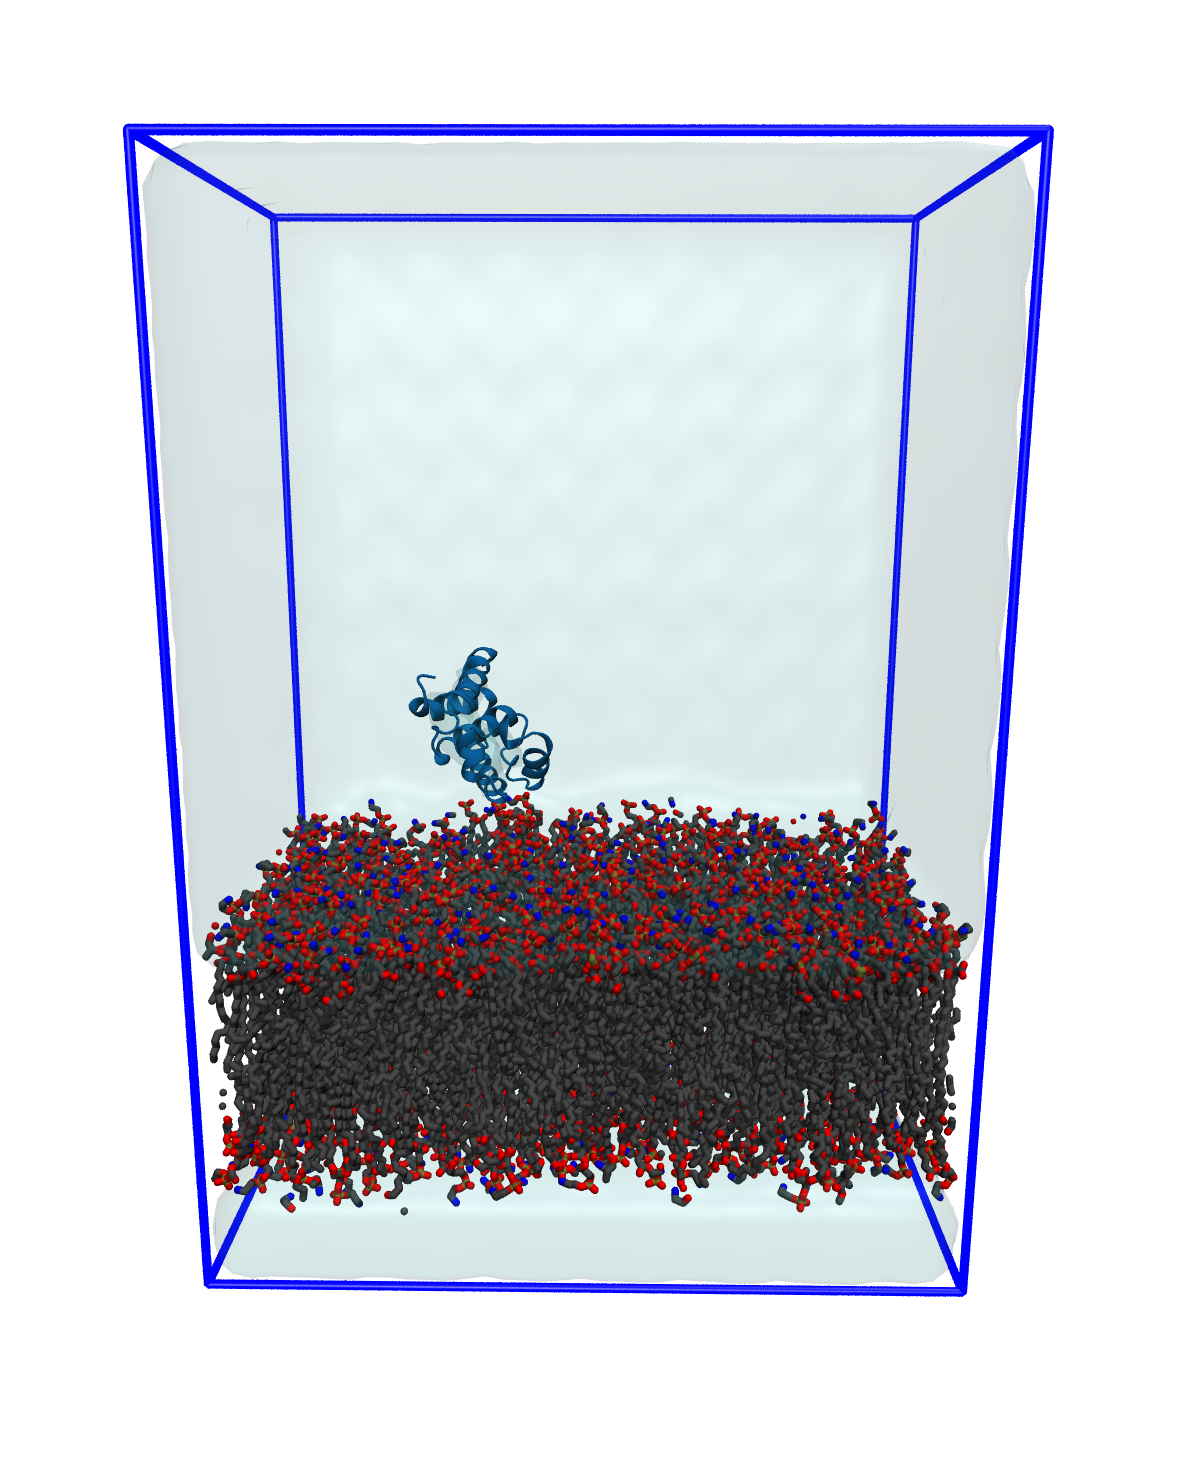
\includegraphics[height=6cm]{figures/setup/setup_umbrella}
	\nicecaption{Setup 2 - Free energy of basic patch}{\charmm{} structure of setup 2. The simulation box comprises the lobe (1936 atoms), one \pip{} (143 atoms) embedded in a \pope{} membrane (509 lipids, 63625 atoms) and water (63199 molecules) which corresponds to 255301 atoms in total. The corresponding \martini{} structure contains 269 beads for the lobe, 6125 beads for the membrane and 16246 water beads. The box dimensions are $14.0\,\si{\nano\metre}$ x $9.0\,\si{\nano\metre}$ x $20.0\,\si{\nano\metre}$.}
	\label{setup:setup2_pic}
\end{figure}
%
%
%
\section{Setup 3 - FAK on a \pip{} membrane}
\label{setup:setup3}
Setup 3 is a \martini{} simulation adopted from \textcite{sara} (\autoref{tobeadded}). It contains a single FAK molecule which was placed on a phosphatidylcholine (\popc{}) and \pip{} membrane (\pip{} concentration $15\%$). NaCl were added to neutralize the system. In contrast to \textcite{sara}, we applied the stabilizing force explained in \autoref{motivation} to the protein.\\
Five independent copies were simulated for $10\,\si{\micro\second}$ each. The temperature was kept at $300\si{\kelvin}$ and the default parameters of \martini{} were used.
%
%
%
\begin{figure}[h]
	\centering
	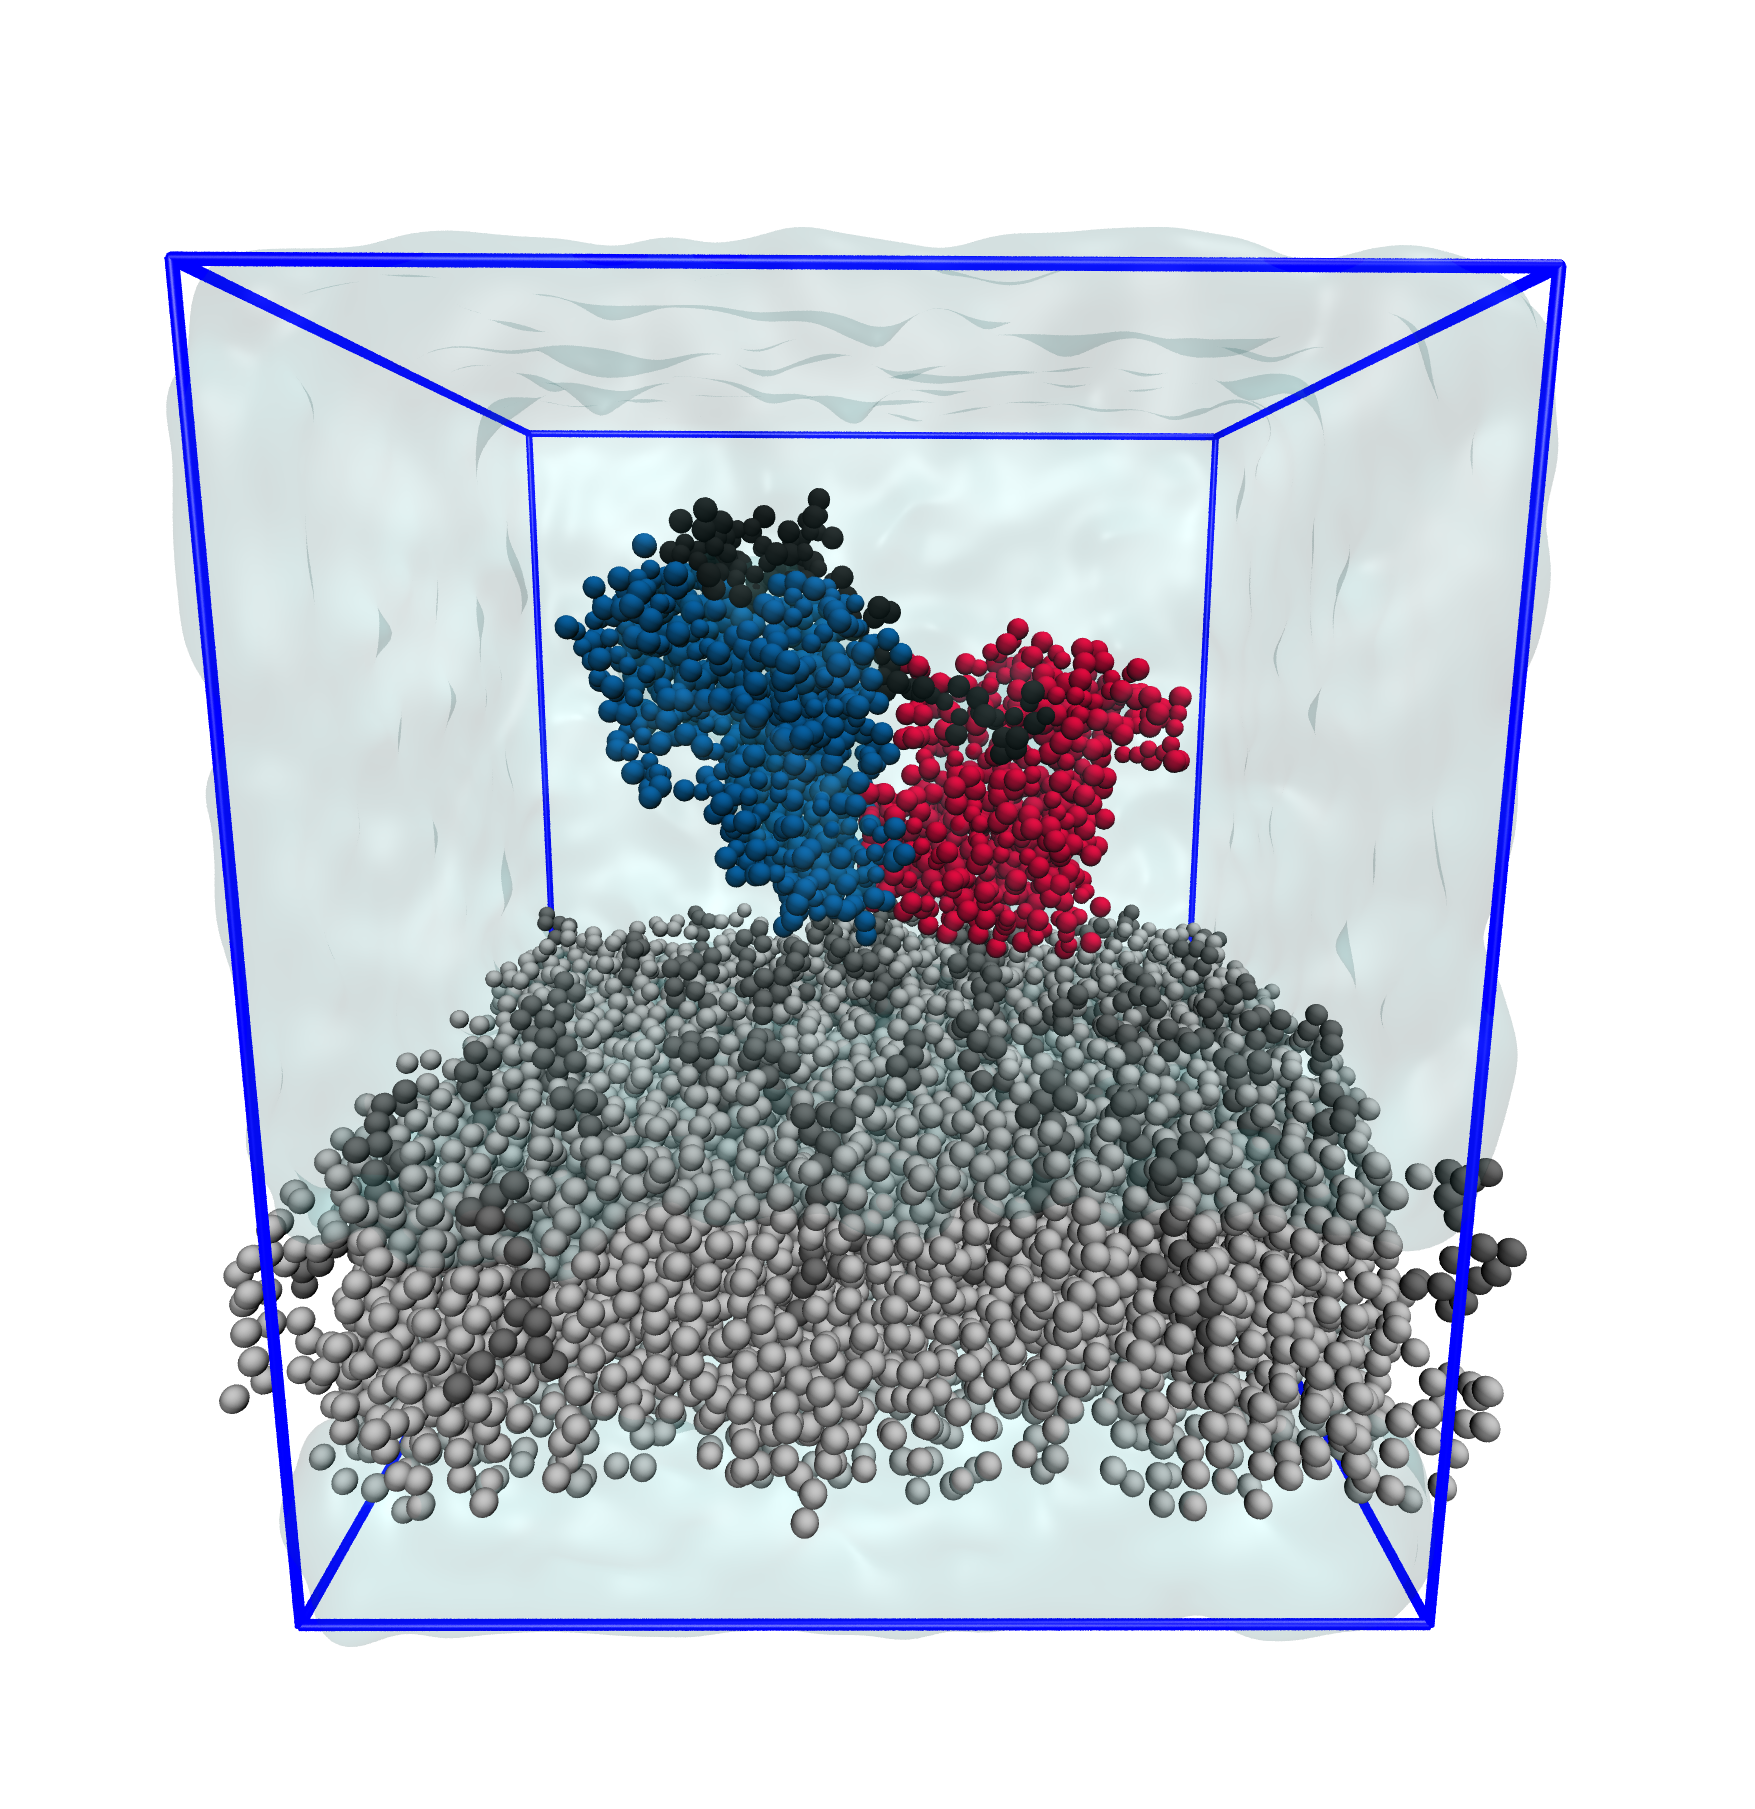
\includegraphics[height=6cm]{figures/setup/setup_gen}
	\nicecaption{Setup 3 - FAK on a \pip{} membrane}{DESCRIPTION NEEDED.}
	\label{setup:setup3_pic}
\end{figure}
%
%
%
\section{Setup 4 - FAK cluster}
From each copy in setup 3, we cut out five frames. All these 25 frames were arranged on a {5x5} grid (\autoref{tobeadded}). Each of the 25 proteins was stabilized with the external force independently. After a short equilibration the system was simulated for $9\,\si{\micro\second}$. We set up 25 different copies, regarding to the arrangement of the frames, resulting in a total simulation time of $45\,\si{\micro\second}$. The temperature was kept at $300\,\si{\kelvin}$ and the default parameters of \martini{} were used.
%
%
%
\begin{figure}[h]
	\centering
	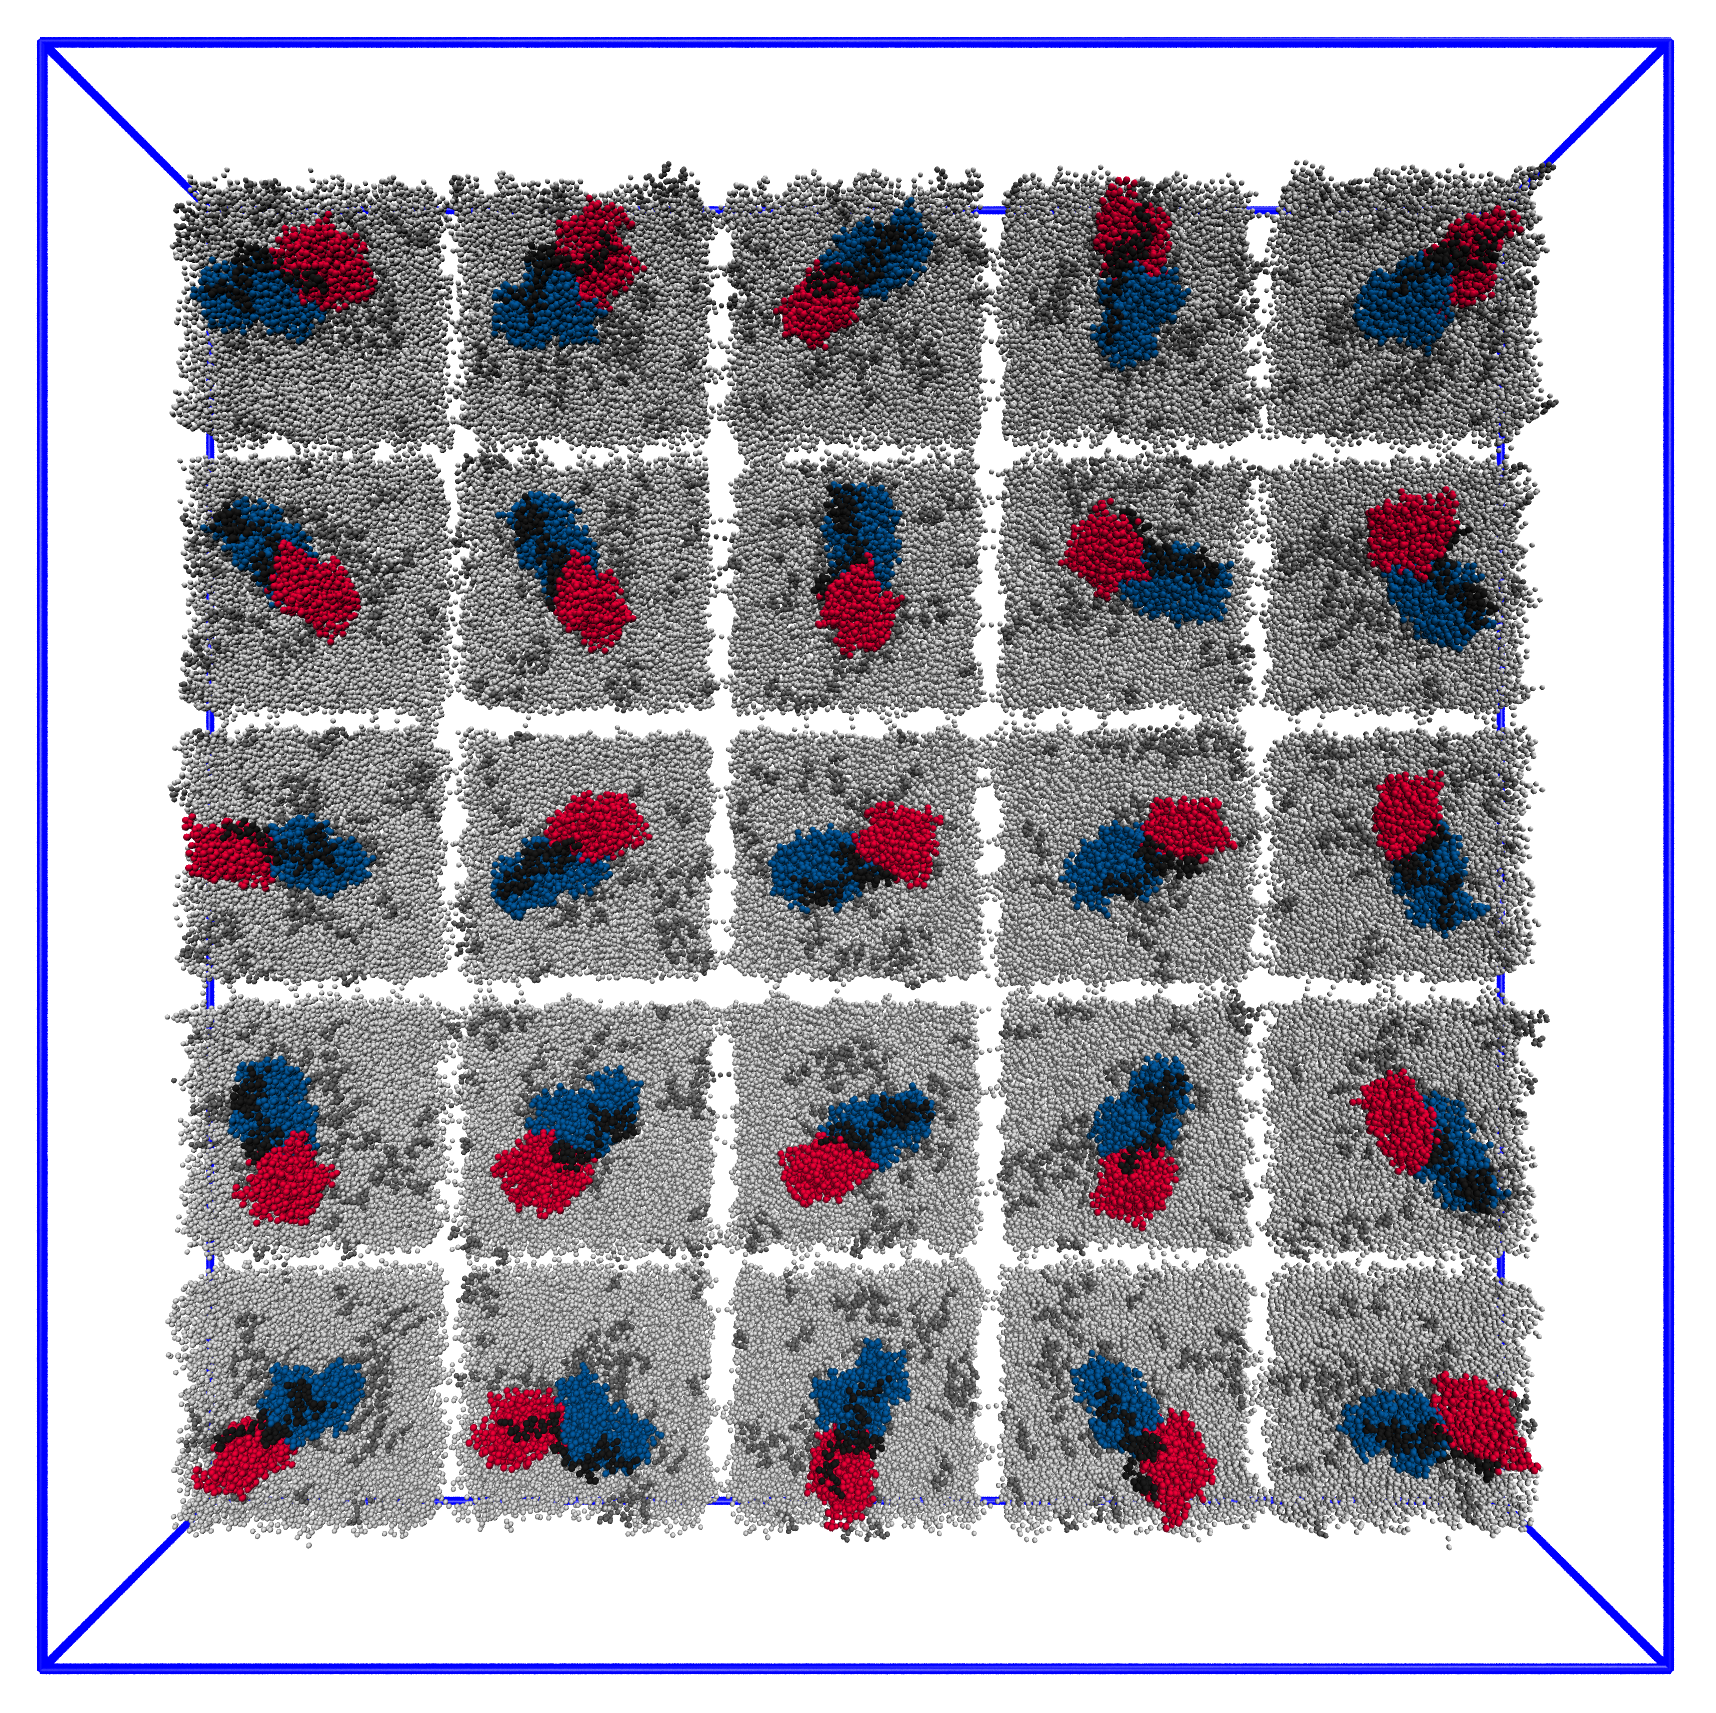
\includegraphics[height=6cm]{figures/setup/setup_cluster}
	\nicecaption{Setup 4 - FAK cluster}{DESCRIPTION NEEDED.}
	\label{setup:setup4_pic}
\end{figure}
%
%
%
%
%
% chapter results
\chapter{Results}
In this chapter we present our results from the simulations. First of all FAK in solution is considered. Afterwards the focus is on the effect of \pip{}. We will start this section with the free energy profile of the basic patch. Since the simulations containing a membrane were carried out with a stabilizing force, we will examine the impact of the force on the observables, before we investigate the conformational changes of FAK induced by binding to the membrane. At the end the results obtained for multiple FAK molecules are presented.
%
%
\section{FAK in solution}
\label{sec:fak_sol}
% TODO: plot 5.1 colorbar frequency, cartoon of spots
In this section, we analyse the conformation of soluted FAK (FAK-SOL) in order to retrieve a reference state for later comparisons. Since the secondary structure of the two domains is fixed due to the elastic network, the focus is on the FERM-kinase interface.\\
\\
The first approach to describe the FERM-kinase interface is to consider the COM distances of F1 to the N-lobe ($d_\text{F1-N}$) and F2 to the C-lobe ($d_\text{F2-C}$).\\
The two dimensional histogram of these distances reveals two different states (see \autoref{free:f2clf1nl}). Spot 1 refers to conformations, which are partially opened at the F2 - C-lobe interface, but close at the F1 - N-lobe interface. In contrast to this, the conformations of spot 2 refers to states in which F2 and the C-lobe gets closer while the distance between F1 and the N-lobe is increased. The corresponding 3D structures are shown in \autoref{free:3d}. They imply that spot 1 refers to a configuration in which the kinase is slightly tilted against the FERM domain while it is in line for configurations associated with spot 2.\\
We observed several transitions between the spots during the simulation, which indicates a sufficiently long simulation time. In total $47.4\%$ of the obtained distances were located in spot 1 and $52.6\%$ in spot 2.\\
\\
A second important quantity associated to the FERM-kinase interface is the contact area (CA) of the interface. However, the observed two state system can not be identified in the CA values (see \autoref{free:ca}), since spot 2 shows only a slightly larger mean value of $27.6\,\si{\nano\metre}^2$ as compared to $27.1\,\si{\nano\metre}^2$ in spot 1.\\
%
%
%
\begin{figure}
	\subcaptionbox{\label{free:f2clf1nl}}[0.49\textwidth]{
		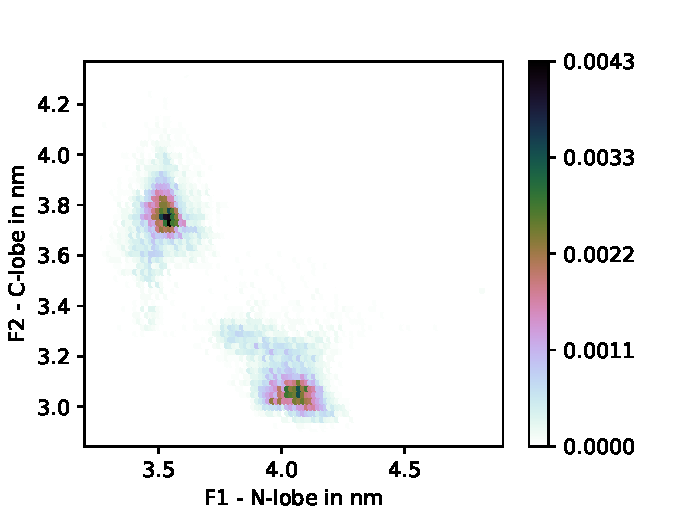
\includegraphics[height=5.2cm]{figures/results/free_f1f2}
	}\hfill%
	\subcaptionbox{\label{free:ca}}[0.49\textwidth]{
		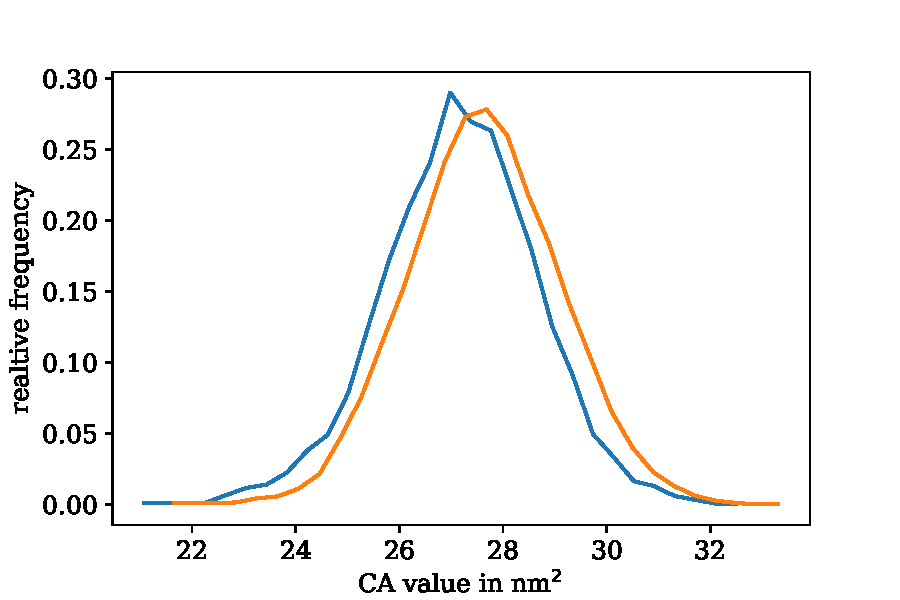
\includegraphics[height=5.2cm]{figures/results/free_ca}
	}%
	\nicecaption{Domain distances and contact area of FAK-SOL}{(\subref{free:f2clf1nl}): two dimensional hexagonal binning plot of $d_\text{F1-N}$ and $d_\text{F2-C}$ which implies a two state system. (\subref{free:ca}): distribution of CA for the two obtained spots.}
\end{figure}
% TODO: label spots
%
%
%
\\
Finally, the contact map showing inter-residue distances of the FERM-kinase interface is considered. Both contact maps, for frames of spot 1 and frames of spot 2, show similar features. Hence, we refer to the contact map of spot 2 in the following. However, since the kinase is tilted against the FERM domain, contacts in area 2 are only observable in frames of spot 2.\\
The average contact map for frames in spot 2 is shown in \autoref{free:contact}. Two regions can be identified. The first one (area 1) is located between F1 and the N-lobe/activation loop. It shows especially contacts between \acid{Y}{576} and \acid{Y}{577} and residues of the FERM domain. The minimal distance in this area, occurring between residue \acid{H}{41} and \acid{Y}{576}, is $0.45\,\si{\nano\metre}$ with an RMSF value of $0.03\,\si{\nano\metre}$. This area reflects the burying of the activity-regulating residues in the closed state (see \autoref{free:3d_spot2}).\\
The second region (area 2, obtained in spot 2 only) is located between F2 and the C-lobe. The spots occur around the residues \acid{Y}{180} and \acid{D}{200} of F2 as well as \acid{F}{596} and \acid{R}{665} of the C-lobe. The minimal distance in this area occurs between \acid{Y}{180} and \acid{F}{596} with $0.45\,\si{\nano\metre}$ and an RMSF value of $0.02\,\si{\nano\metre}$. Mutation experiments showed these two residues to have an important effect upon the interface \autocite{structFAK}, which fits to these observations.\\
The linker shows contacts with both domains. The minimal distances in the marked areas occur between the autophosphorylation site \acid{Y}{397} and \acid{H}{58} of F1 ($0.45\,\si{\nano\metre}$, RMSF $0.03\,\si{\nano\metre}$) as well as \acid{Y}{397} and \acid{Y}{576} of the kinase ($0.50\,\si{\nano\metre}$, RMSF $0.10\,\si{\nano\metre}$). Furthermore, several interactions occur between the residues in the linker itself, namely, between \acid{S}{379} to \acid{V}{389} and \acid{T}{394} to \acid{I}{400} (area 5). Also in this spot, the minimal distance occurs between \acid{Y}{397} and \acid{T}{386} ($0.52\,\si{\nano\metre}$, RMSF $0.04\,\si{\nano\metre}$). The density in this area implies that the linker forms a ball, which is slightly plunged into the interface of the FERM domain and the kinase (regarding area 3 and area 4). This can be seen also in the 3D structure in \autoref{free:3d_spot2}. Our observations support the thesis that autophosphorylation is prevented in the closed conformation by a binding of the linker to the FERM domain \autocite{pap003}.\\
%
%
\begin{figure}
	\centering
	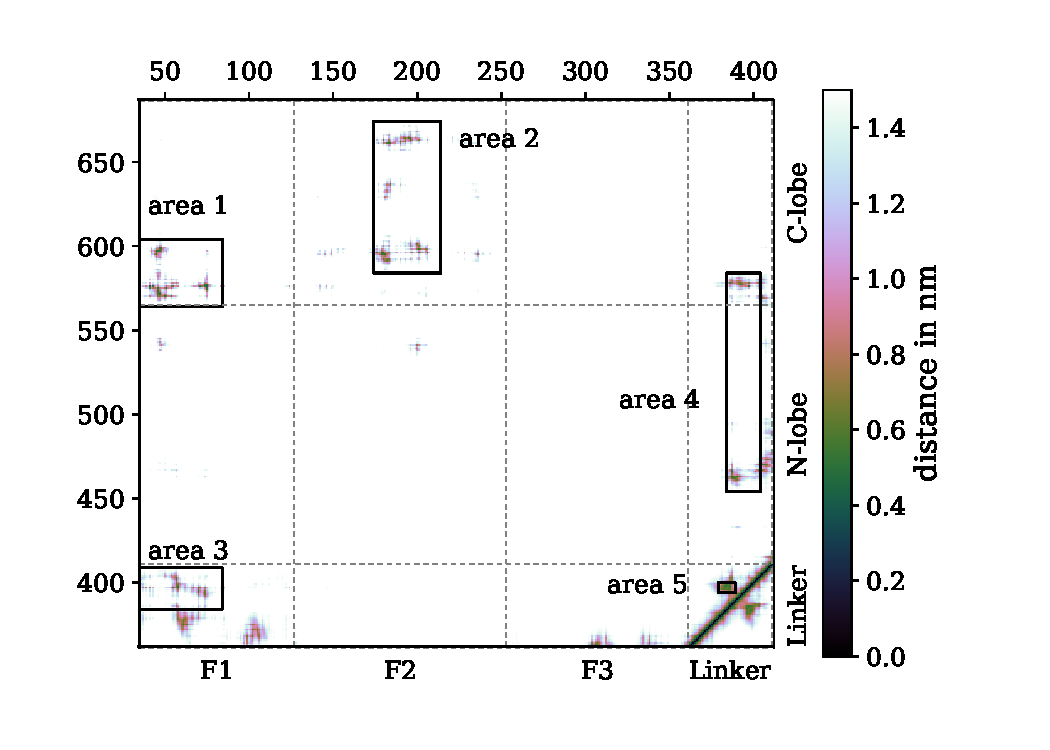
\includegraphics[width=.8\textwidth]{figures/results/contactmap_free}
	\nicecaption{Contact map of FAK-SOL}{Average contact map of the FERM-kinase interface and the linker region for frames of spot 2. The contact map for frames of spot 1 is similar, but lacks the contacts in area 2. In the contact map the burying of the active site (area 1) as well as the hiding of the autophosphorylation site \acid{Y}{397} (area 3, 4 and 5) can be seen.}
	\label{free:contact}
\end{figure}
%
%
%
%
%
%
\begin{figure}
	\subcaptionbox{\label{free:3d_spot1}}[0.32\textwidth]{
		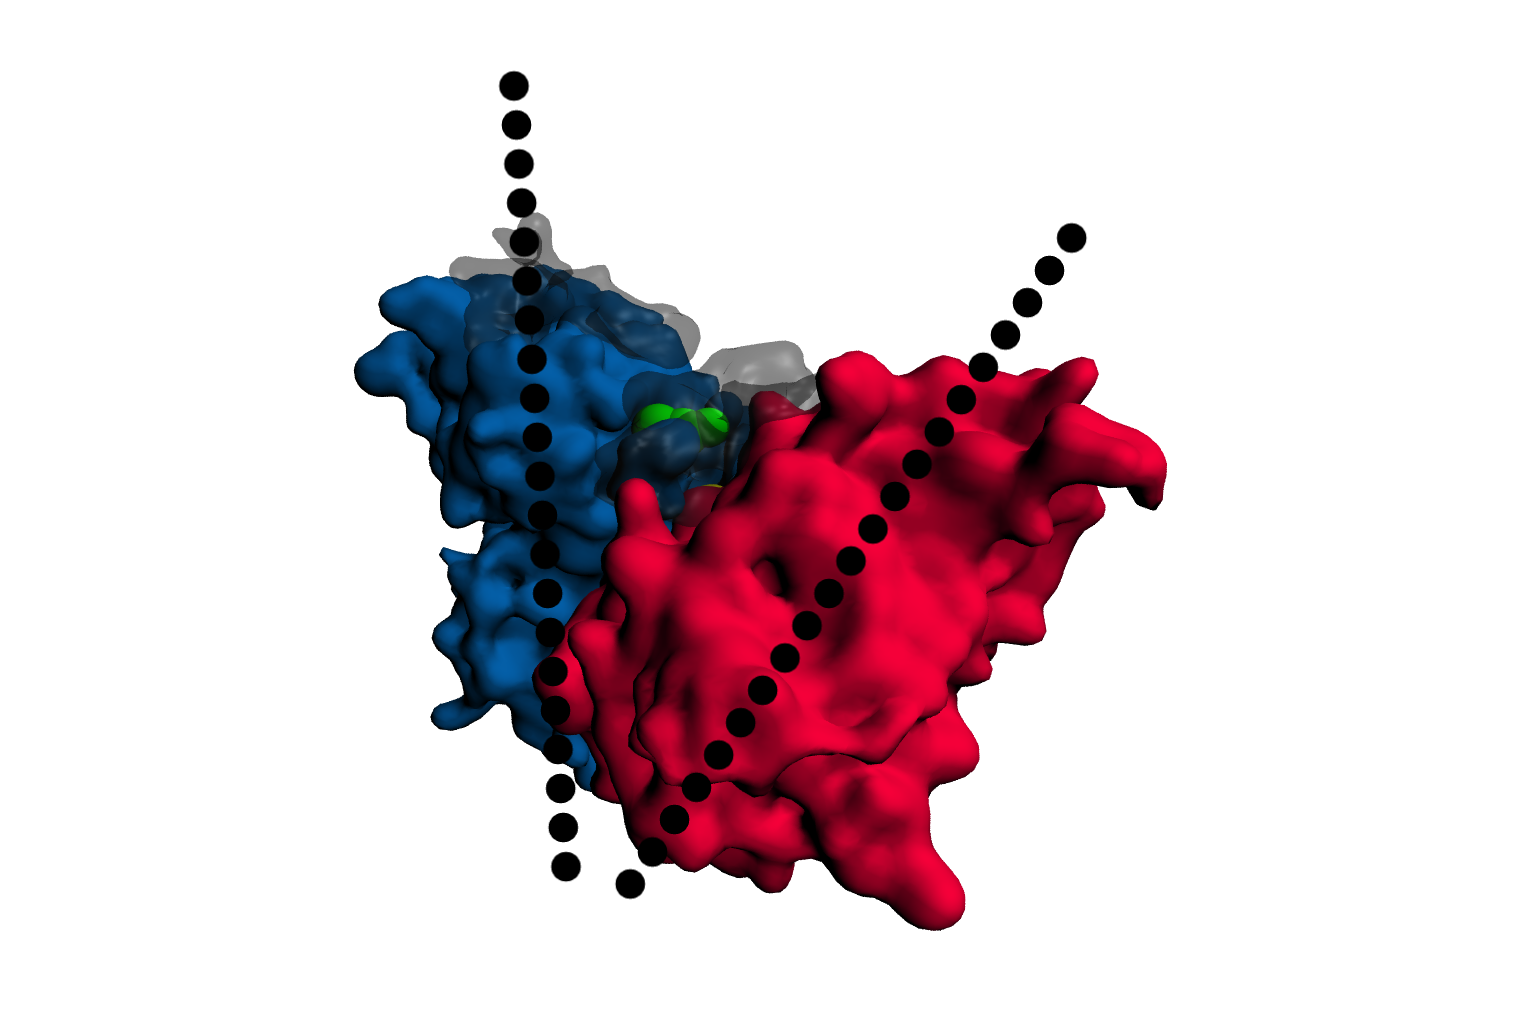
\includegraphics[height=4cm]{figures/results/fak_spot1}
	}\hfill%
	\subcaptionbox{\label{free:3d_spot2}}[0.32\textwidth]{
		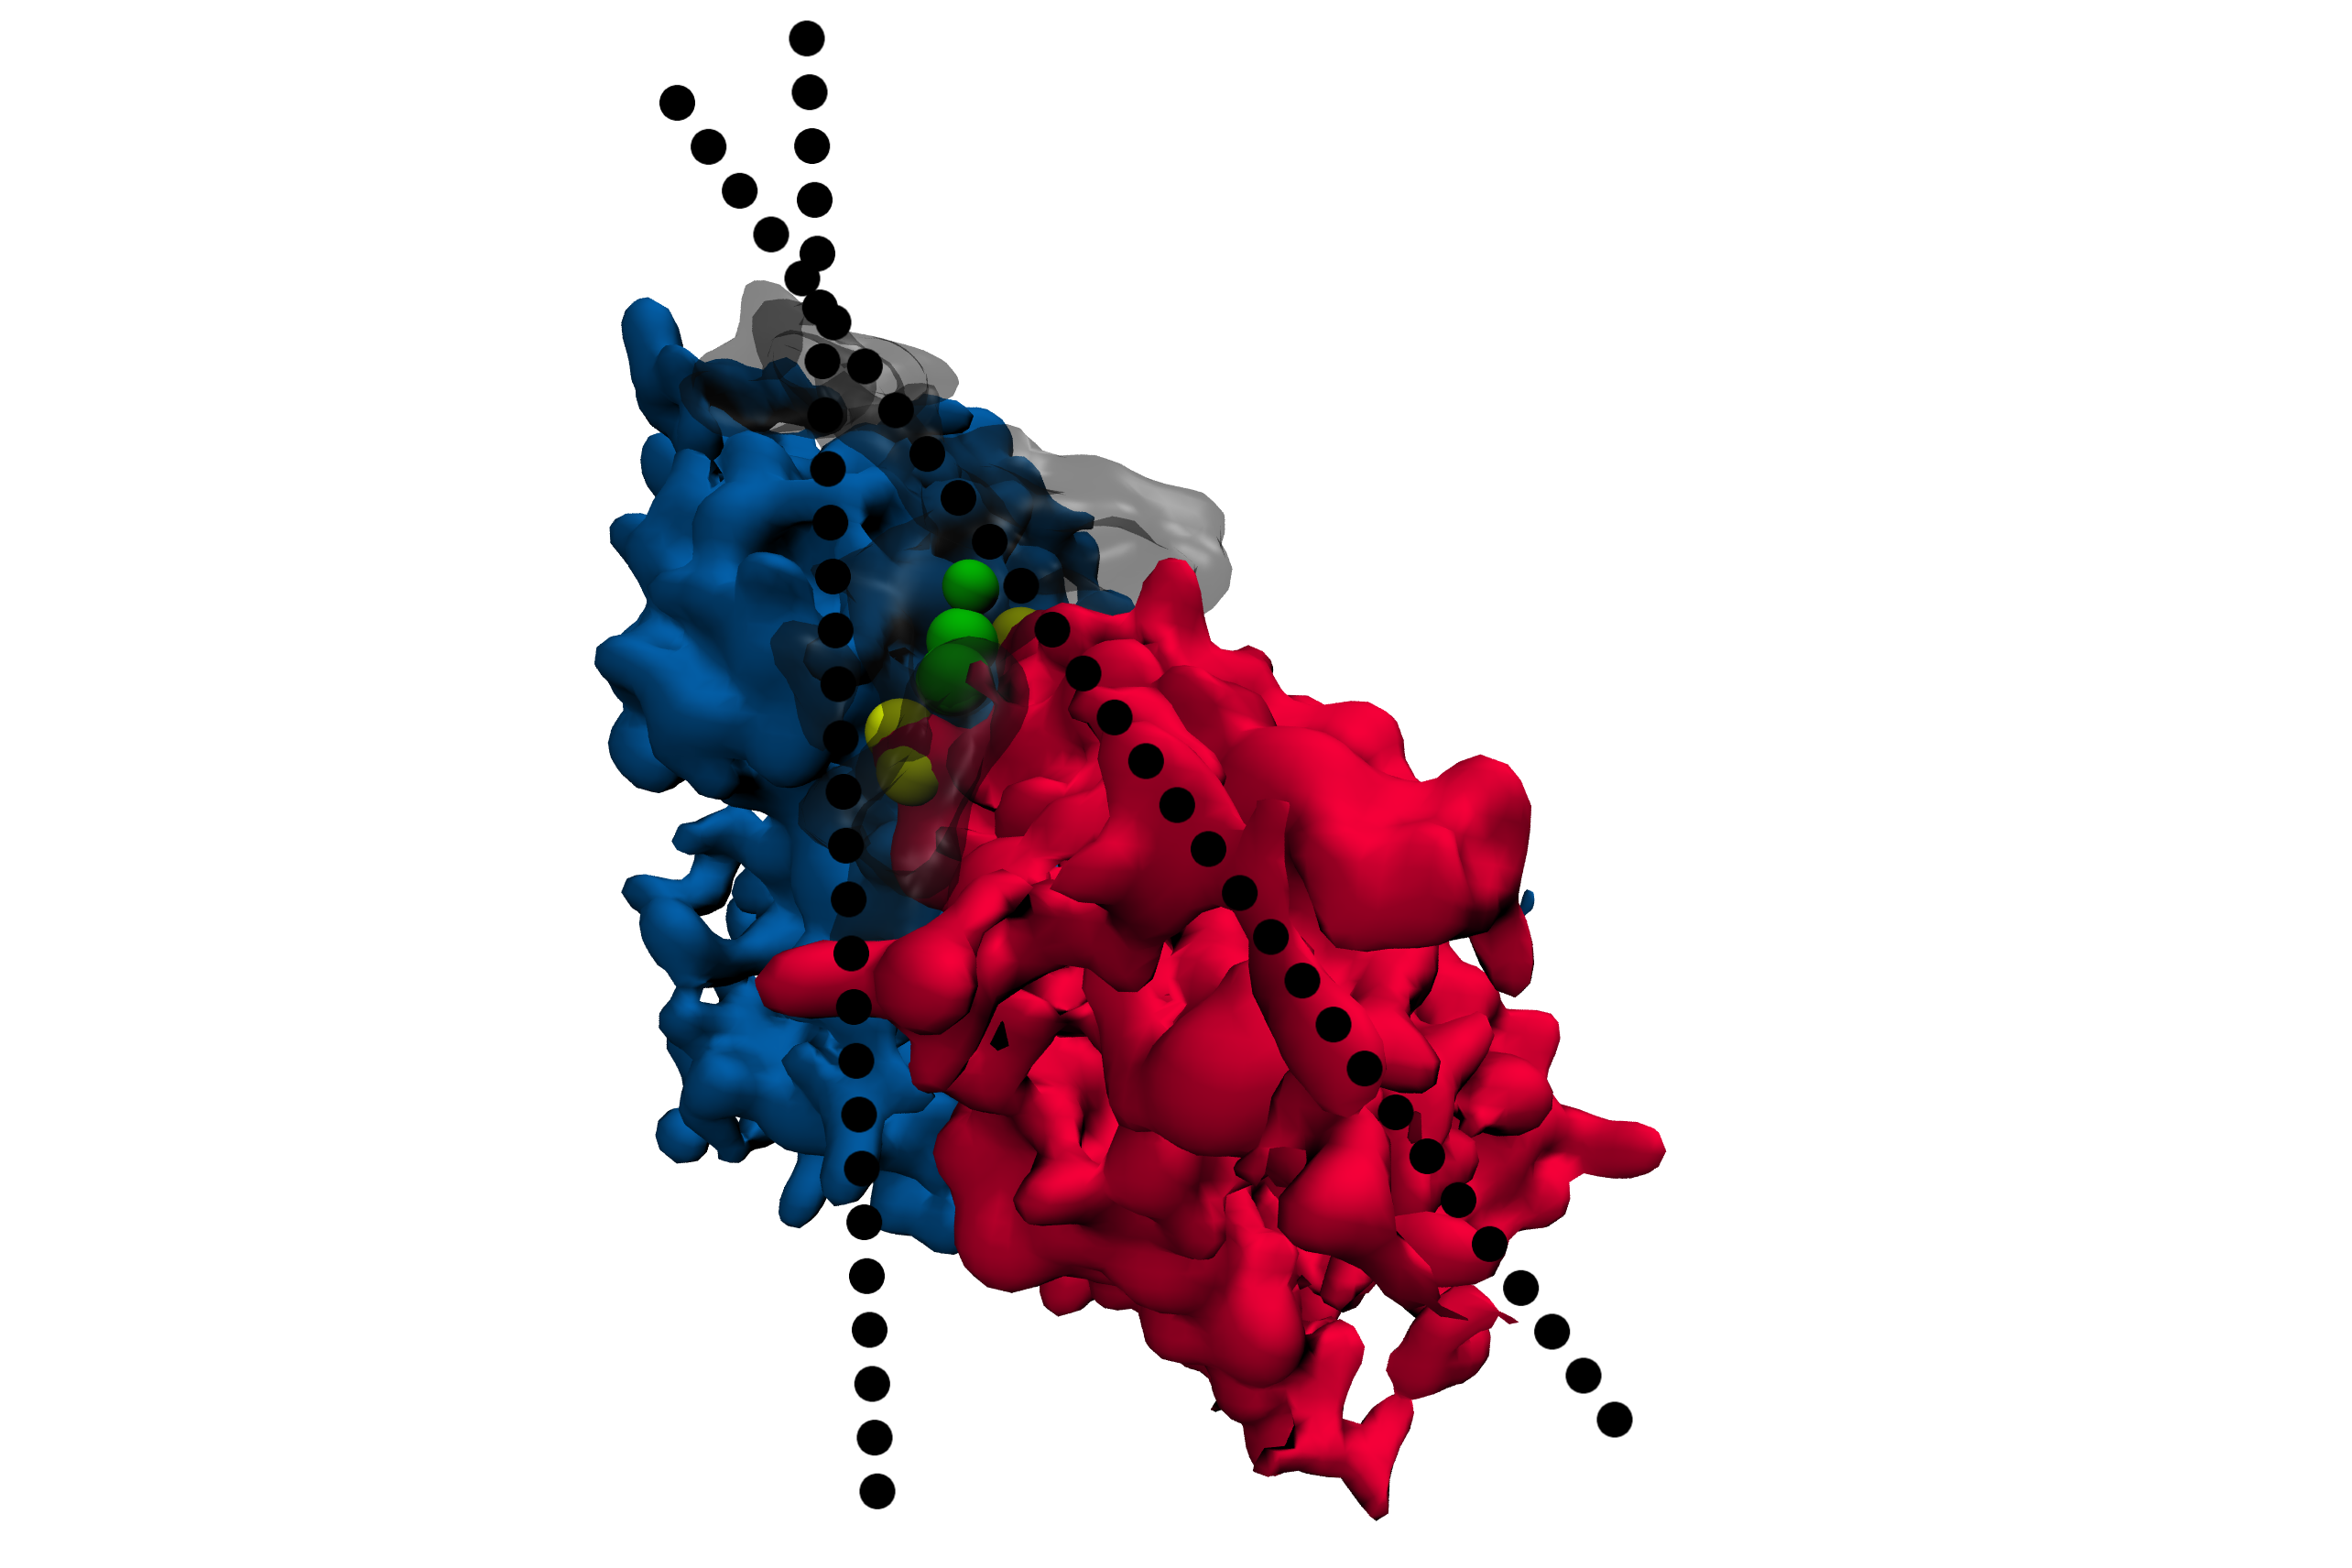
\includegraphics[height=3.5cm]{figures/results/fak_spot2}
	}\hfill%
	\subcaptionbox{\label{free:3d_spot_top}}[0.32\textwidth]{
		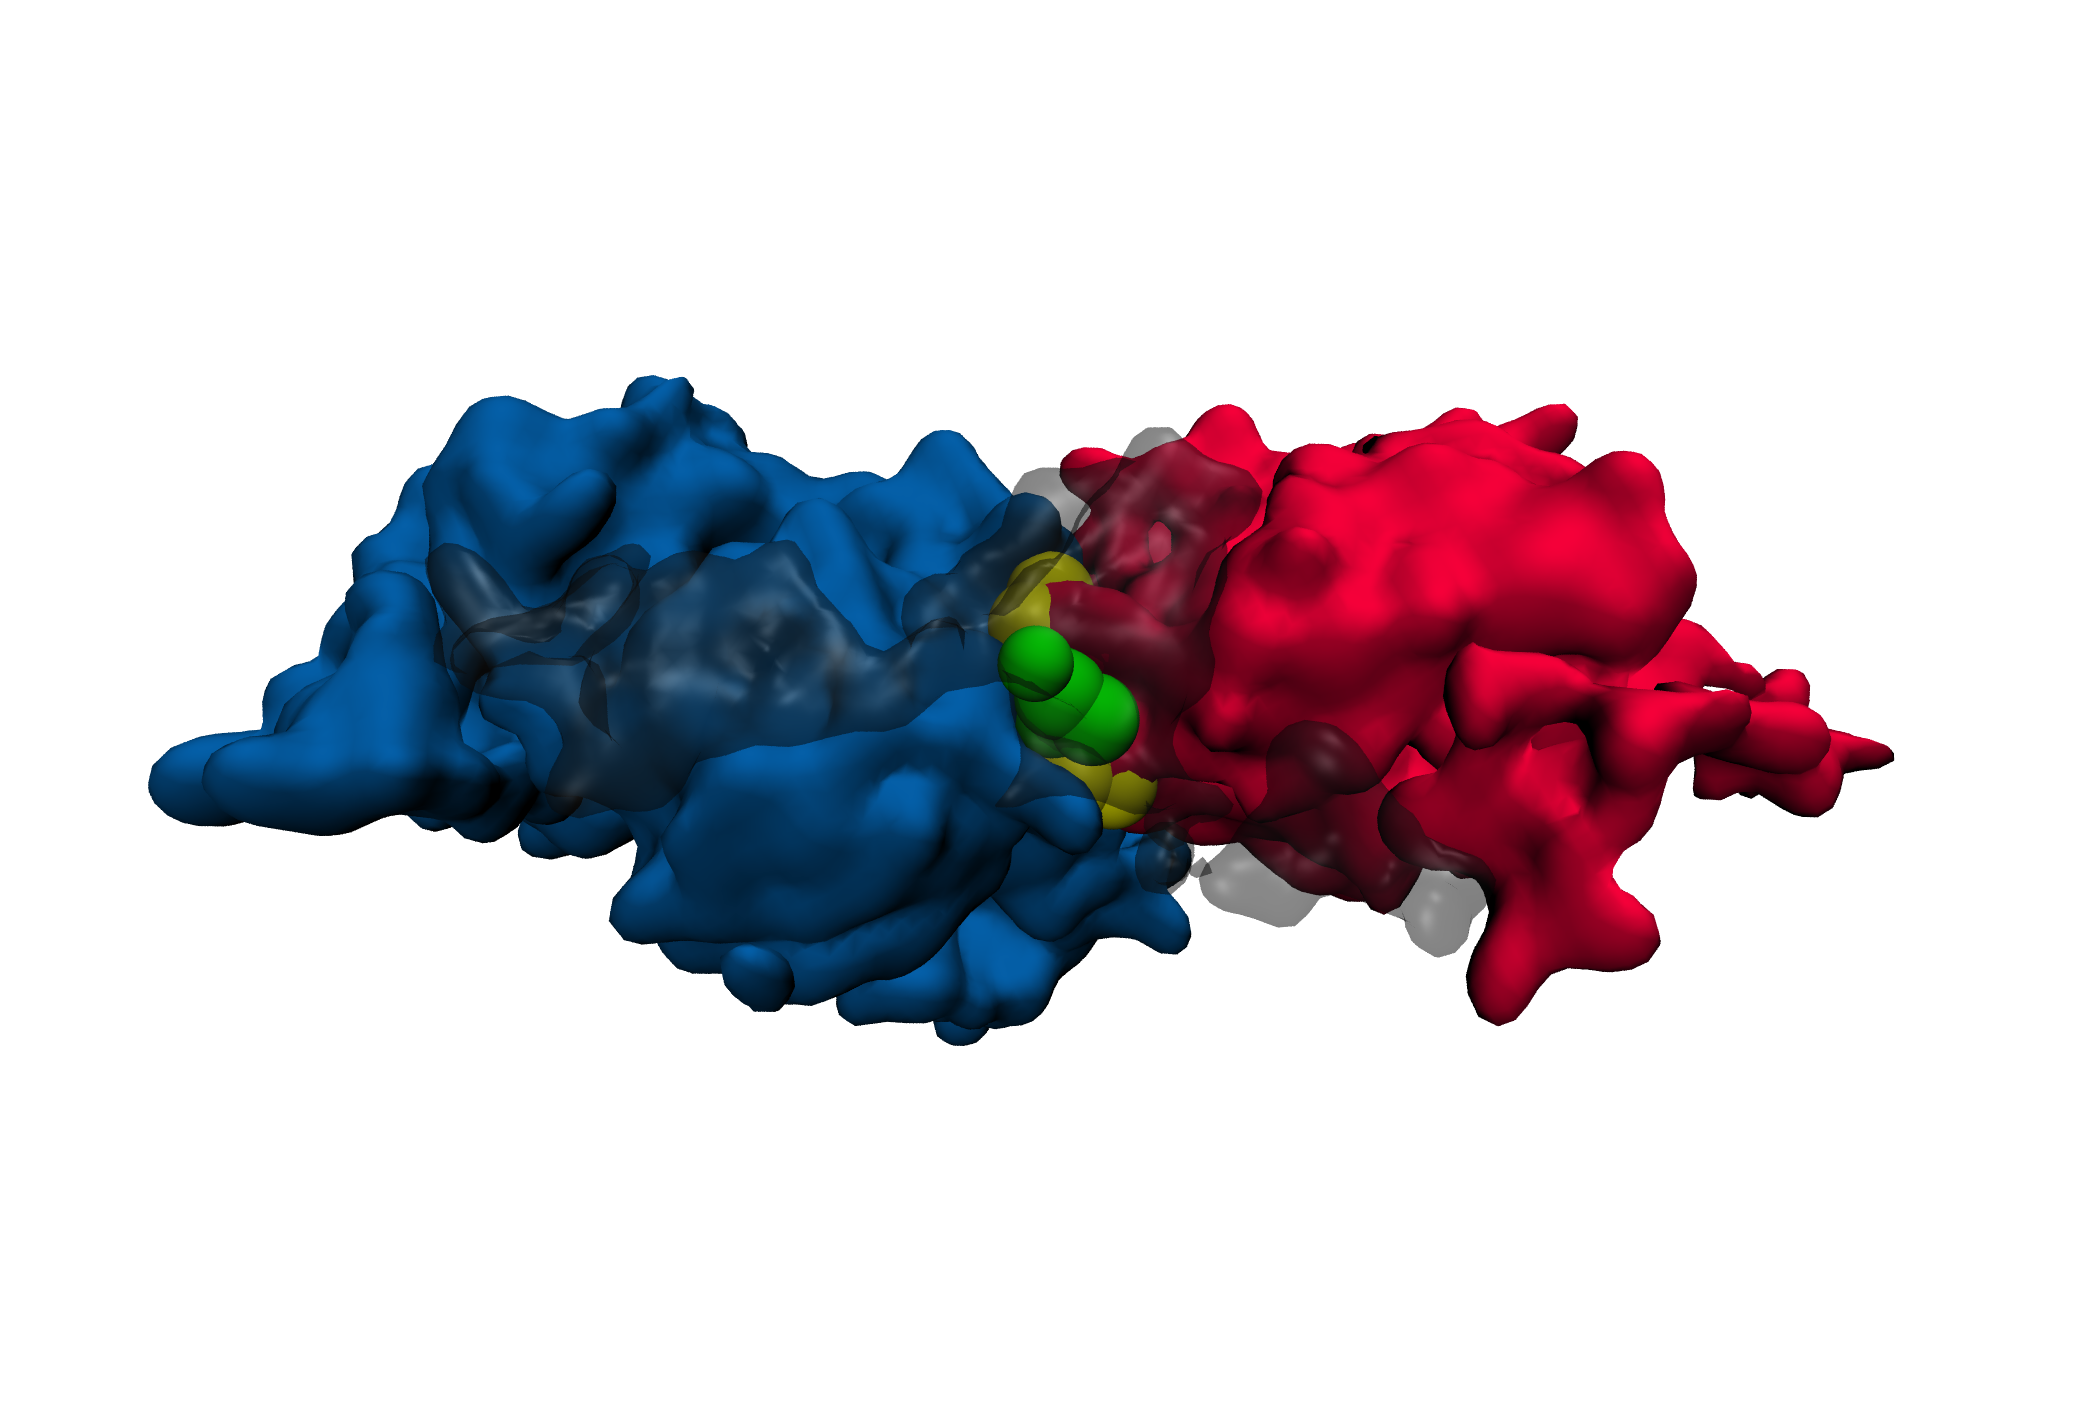
\includegraphics[height=3.5cm]{figures/results/fak_spot2_top}
	}
	\nicecaption{3D structure of the two states in FAK-SOL}{The 3D structures show the FERM domain (blue), the kinase (red) and the linker (black, transparent). The autophosphorylation site \acid{Y}{397} (green) is plunged into the interface and hidden by the linker. \acid{Y}{576} and \acid{Y}{577} (yellow) are shielded by the FERM domain.\\
	(\subref{free:3d_spot1}, spot 1): The kinase is tilted against FERM. (\subref{free:3d_spot2}, spot 2): Both domains are in line. (\subref{free:3d_spot_top}, spot 2): \acid{Y}{397}, \acid{Y}{576} and \acid{Y}{577} are shielded by the linker.}
\label{free:3d}
\end{figure}
%
%
%

%
%
\section{Free energy profile of basic patch}
\label{results:umbrella}
In order to understand the falling of FAK onto the membrane the free energy profile of the binding of the basic patch to \pip{} was investigated. Since this binding is the main contact between FAK and the membrane in our model, a short report on the results is given at this point.\\
The profiles are obtained from setup 2. The reaction coordinate is the z component of the COM distance between \pip{} and the protein fragment. For each forcefield, C36, \martini{} and \martini{} with PW, the average profile out of the five copies together with the standard deviation can be found in \autoref{umbrella:profiles}. The range $6\,\si{\nano\metre} \le z \le 7\,\si{\nano\metre}$ was set as zero point.\\
%
%
%
\begin{figure}[hb]
	\centering
	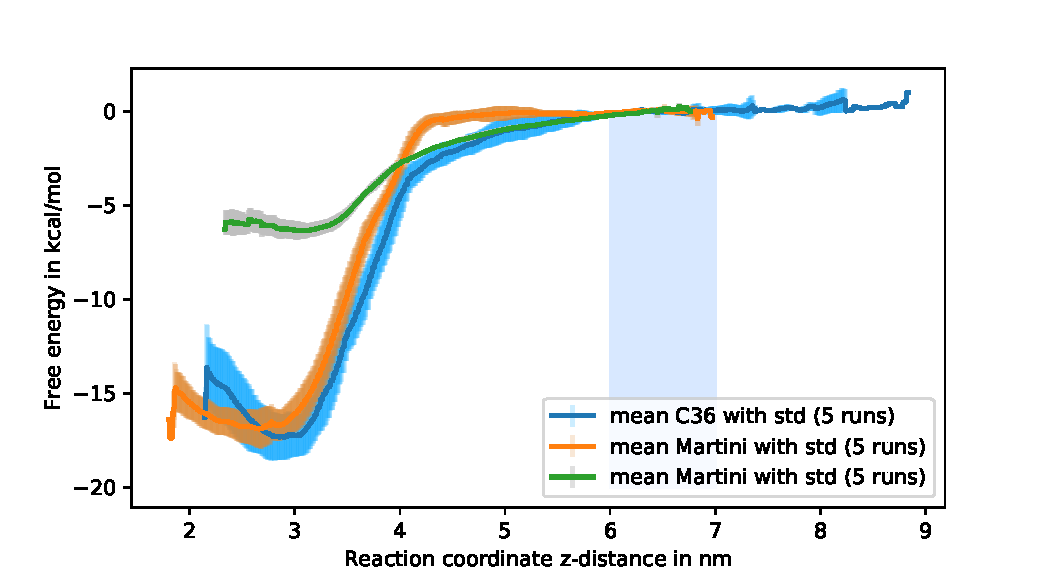
\includegraphics[width=.8\textwidth]{figures/results/umbrella}
	\nicecaption{Free energy profile of basic patch}{For each forcefield the average and standard deviation of the five copies is presented.}
	\label{umbrella:profiles}
\end{figure}
%
%
%
\\
Both, C36 and \martini{}, show a similar energy depth of $\approx 17 \si{\kilo Cal/\mole}$ and a similar slope between $3\,\si{\nano\metre} \le z \le 4\,\si{\nano\metre}$ . Certainly, \martini{} shows systematically more shallow wells than the all atom simulation. This can be attributed to the proposed underestimation of electrostatic forces due to the unpolar water beads (see \autoref{subsub:coarsegraining}). The difference at $z = 4.2\,\si{\nano\metre}$ originates from the different treatment of long range electrostatics: \martini{} uses a cut-off radius, C36 uses PME.\\ %TODO: maybe force switch function in martini? what about the kink in C36?
Also \martini{} with PW uses PME for long range electrostatic interactions and indeed it fits much better to the C36 profile for larger distances. However, the binding strength is crucially underestimated in Martini with PW.\\
The extent to which \martini{} reproduces the results from all-atom simulations is remarkable, even though the parameters for \martini{} were obtained from free energy calculations (see \autoref{subsub:coarsegraining})\\
\\
In the used starting configurations, the proteins are already bound to \pip{}. Therefore a correct binding strength and the shape near the minimum is of larger interest than a correct sampling of farther distances. In addition \martini{} with PW required a much higher computational effort. That is why we consider only the standard water model in the following simulations.

%
%
\section{Impact of stabilizing force}
\subsection{Impacts of the stabilizing force}
In setup 3 a and setup 4 each protein was stabilized with an external force acting on the FERM domain (see \autoref{motivation}). Therefore the dependency of the used observables is examined below.\\
\\
The force has a mean value of $1.47\,\forceunit$ and a standard deviation of $13.13\,\forceunit$. It is skewed to positive values. This is expected since positive values of the force require negative elongations $\Delta z$. If the connecting vector of F1 and F2 $\vec{d}_F$ is parallel to the z-axis, larger negative deviations require a stretching of $d_F$, which suppress these forces. \\
\\
Linear regressions show that none of the quantities $d_F$, $d_\text{F1-N}$, $d_\text{F2-C}$ and CA have a remarkable correlation to the applied force. Here remarkable means that either the regression result was not significant or that the obtained slope was so small, that a change of two standard deviations in force would not change the quantity noticeably.\\
\\
Also the distances between residue pairs are tested for correlation with the applied force. To this end, 10 different proteins without neighbours were picked out of the trajectories of setup 4, each for $1\,\si{\micro\second}$. On this dataset a linear regression was performed for each residue pair. \autoref{force:contactmap} shows the calculated Pearson correlation coefficient (only significant correlations with Pearson $\left|r\right| > 0.3$). The mean value of the slope for the positive correlated pair distances is $20.3\,\si{\pico\newton/\nano\metre}$ and $-19.7\,\si{\pico\newton/\nano\metre}$ for the negative correlated pair distances. Thus, the force can have large influences on these pairs. However, not all observed contacts at the interface (compare to \autoref{free:contact}) are effected.
%
%
%
\begin{figure}
	\centering
	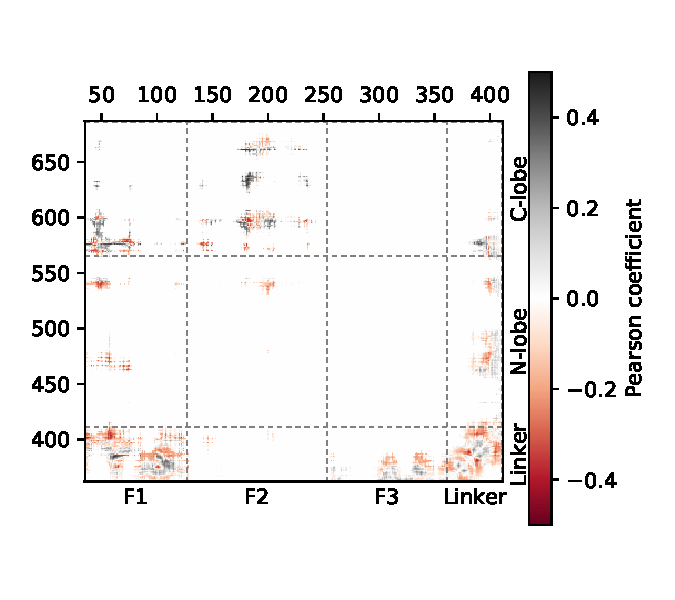
\includegraphics[width=.7\textwidth]{figures/results/interface_corr}
	\nicecaption{Correlations in contact map}{The contact map shows residue pairs, whose distance correlates with the applied force. The obtained slope is about $20\,\si{\pico\newton/\nano\metre}$.}
	\label{force:contactmap}
\end{figure}
%
%
%
\\
It is important to note that in this section only the observed quantities were tested for correlation with the force. It is however possible and probable, that due to this restriction, configurations or states are completely missing while others are over expressed. This effect can not be estimated, but should be kept in mind.
%
%
\section{Conformational changes on a membrane}
In this section, the conformation of FAK bound to a \pip{} containing membrane (FAK-MEM) is compared to the observations of FAK-SOL. To this end, FAK structures of setup 4 were used with the condition that the FAK molecules have no neighbours. The contact map is based on the same dataset which was used for \autoref{force:contactmap}.\\
\\
The distribution of $d_\text{F2-C}$ shown in \autoref{mem:comdist} lacks the peak observed for FAK-SOL at $3.8\,\si{\nano\metre}$ which has been associated with spot 1. Also the distribution of $d_\text{F1-N}$ shows a distinct peak at values associated to spot 2 observed in FAK-SOL ($4.0\,\si{\nano\metre}$). This induces that the tilting of the kinase domain is suppressed in presence of the membrane which is reasonable since both, FERM domain and kinase have a docking site for \pip{}. However, there is a significant increase in the contact area (\autoref{mem:contactarea}) to $30.8\,\si{\nano\metre}^2$. Therefore, we analysed the FERM-kinase interface in order to get a more detailed insight in the conformational change.\\
\\
The contact map in \autoref{mem:contact} shows the difference to the contact map obtained for FAK-SOL. At the interface of F2 and the C-lobe (area 1) the residue distances get closer. In area 2 both, increasing and decreasing distances can be found. Regarding the 3D structure (\autoref{mem:3d}) one can see that although the upper part of the interface (contacts between \acid{P}{49} to \acid{S}{54} and the kinase) gets closer, the region below (contacts between \acid{E}{44} to \acid{E}{48} and the kinase) gets farther away. This induces a spreading of the interface at the activation loop including the activity regulating residues \acid{Y}{576} and \acid{Y}{577}.\\
Also in the linker region conformational changes can be observed. Area 3 indicates that the ball structure of the \acid{Y}{397} containing ball structure observed in FAK-SOL disappears. As shown in \autoref{mem:3d} the linker is pulled back to the FERM domain which results in an exposed position of the autophosphorylation site \acid{Y}{397}.\\
\\
As suggested by findings of \textcite{pap001} and \textcite{pap003} the FERM domain does not dissociate from the kinase because of binding to \pip{}. However this binding leads to conformational changes resulting in a partial opening of the FERM kinase interface and the exposure of the autophosphorylation site \acid{Y}{397}.
%
%
%
\begin{figure}
	\subcaptionbox{\label{mem:comdist}}[0.49\textwidth]{
		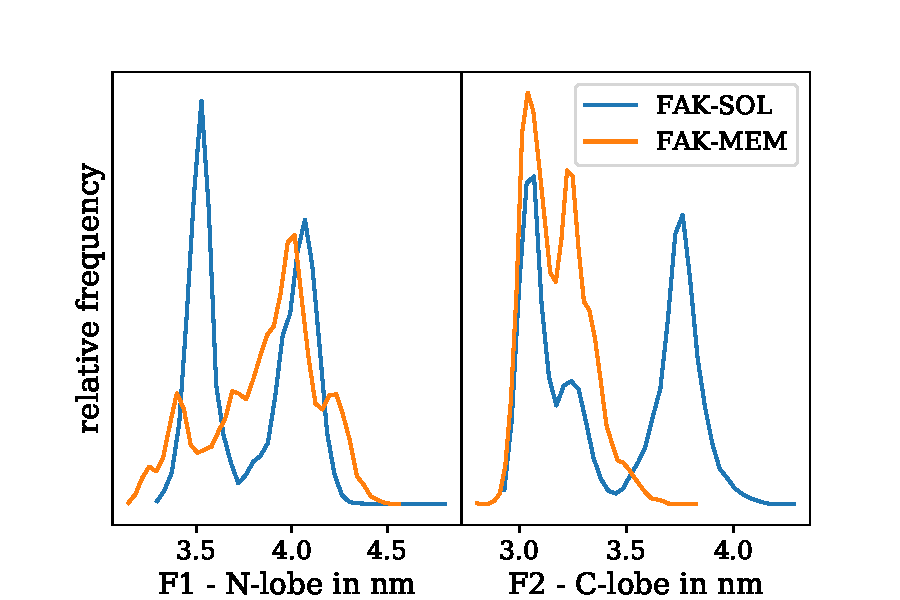
\includegraphics[height=5cm]{figures/results/comp_free_mem_comdist}
	}\hfill%
	\subcaptionbox{\label{mem:contactarea}}[0.49\textwidth]{
		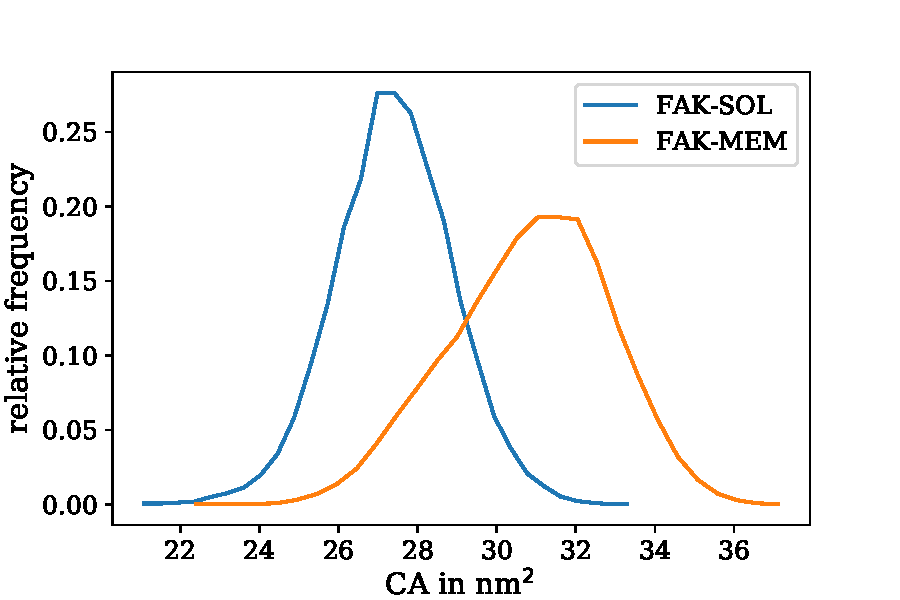
\includegraphics[height=5cm]{figures/results/ca_sol_mem}
	}%
	\nicecaption{Domain distances and contact area of FAK-MEM}{(\subref{mem:comdist}): distribution of $d_\text{F1-N}$ and $d_\text{F2-C}$ in comparison to FAK-SOL. (\subref{mem:contactarea}): contact area in comparison to FAK-SOL}
\end{figure}
%
%
%
%
%
%
\begin{figure}
	\centering
	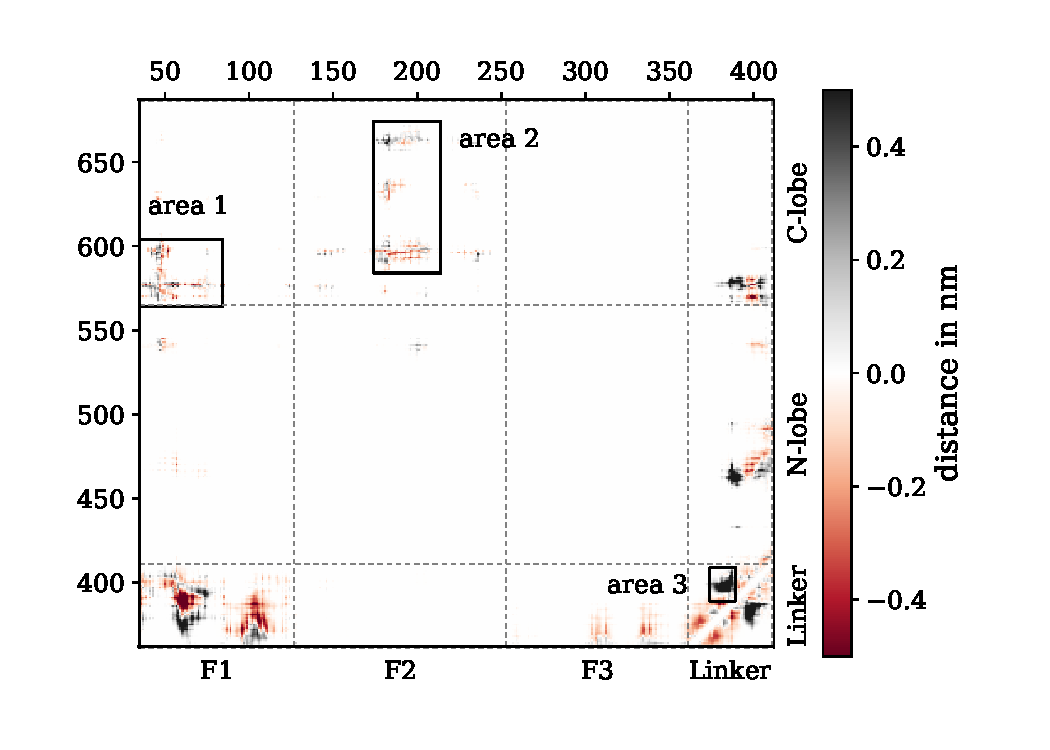
\includegraphics[width=.8\textwidth]{figures/results/contactmap_diff_to_free}
	\nicecaption{Contact map of FAK-MEM}{The contact map shows the difference FAK-MEM - FAK-SOL of the inter-residue distances.}
	\label{mem:contact}
\end{figure}
%
%
%
%
%
%
\begin{figure}
	\centering
	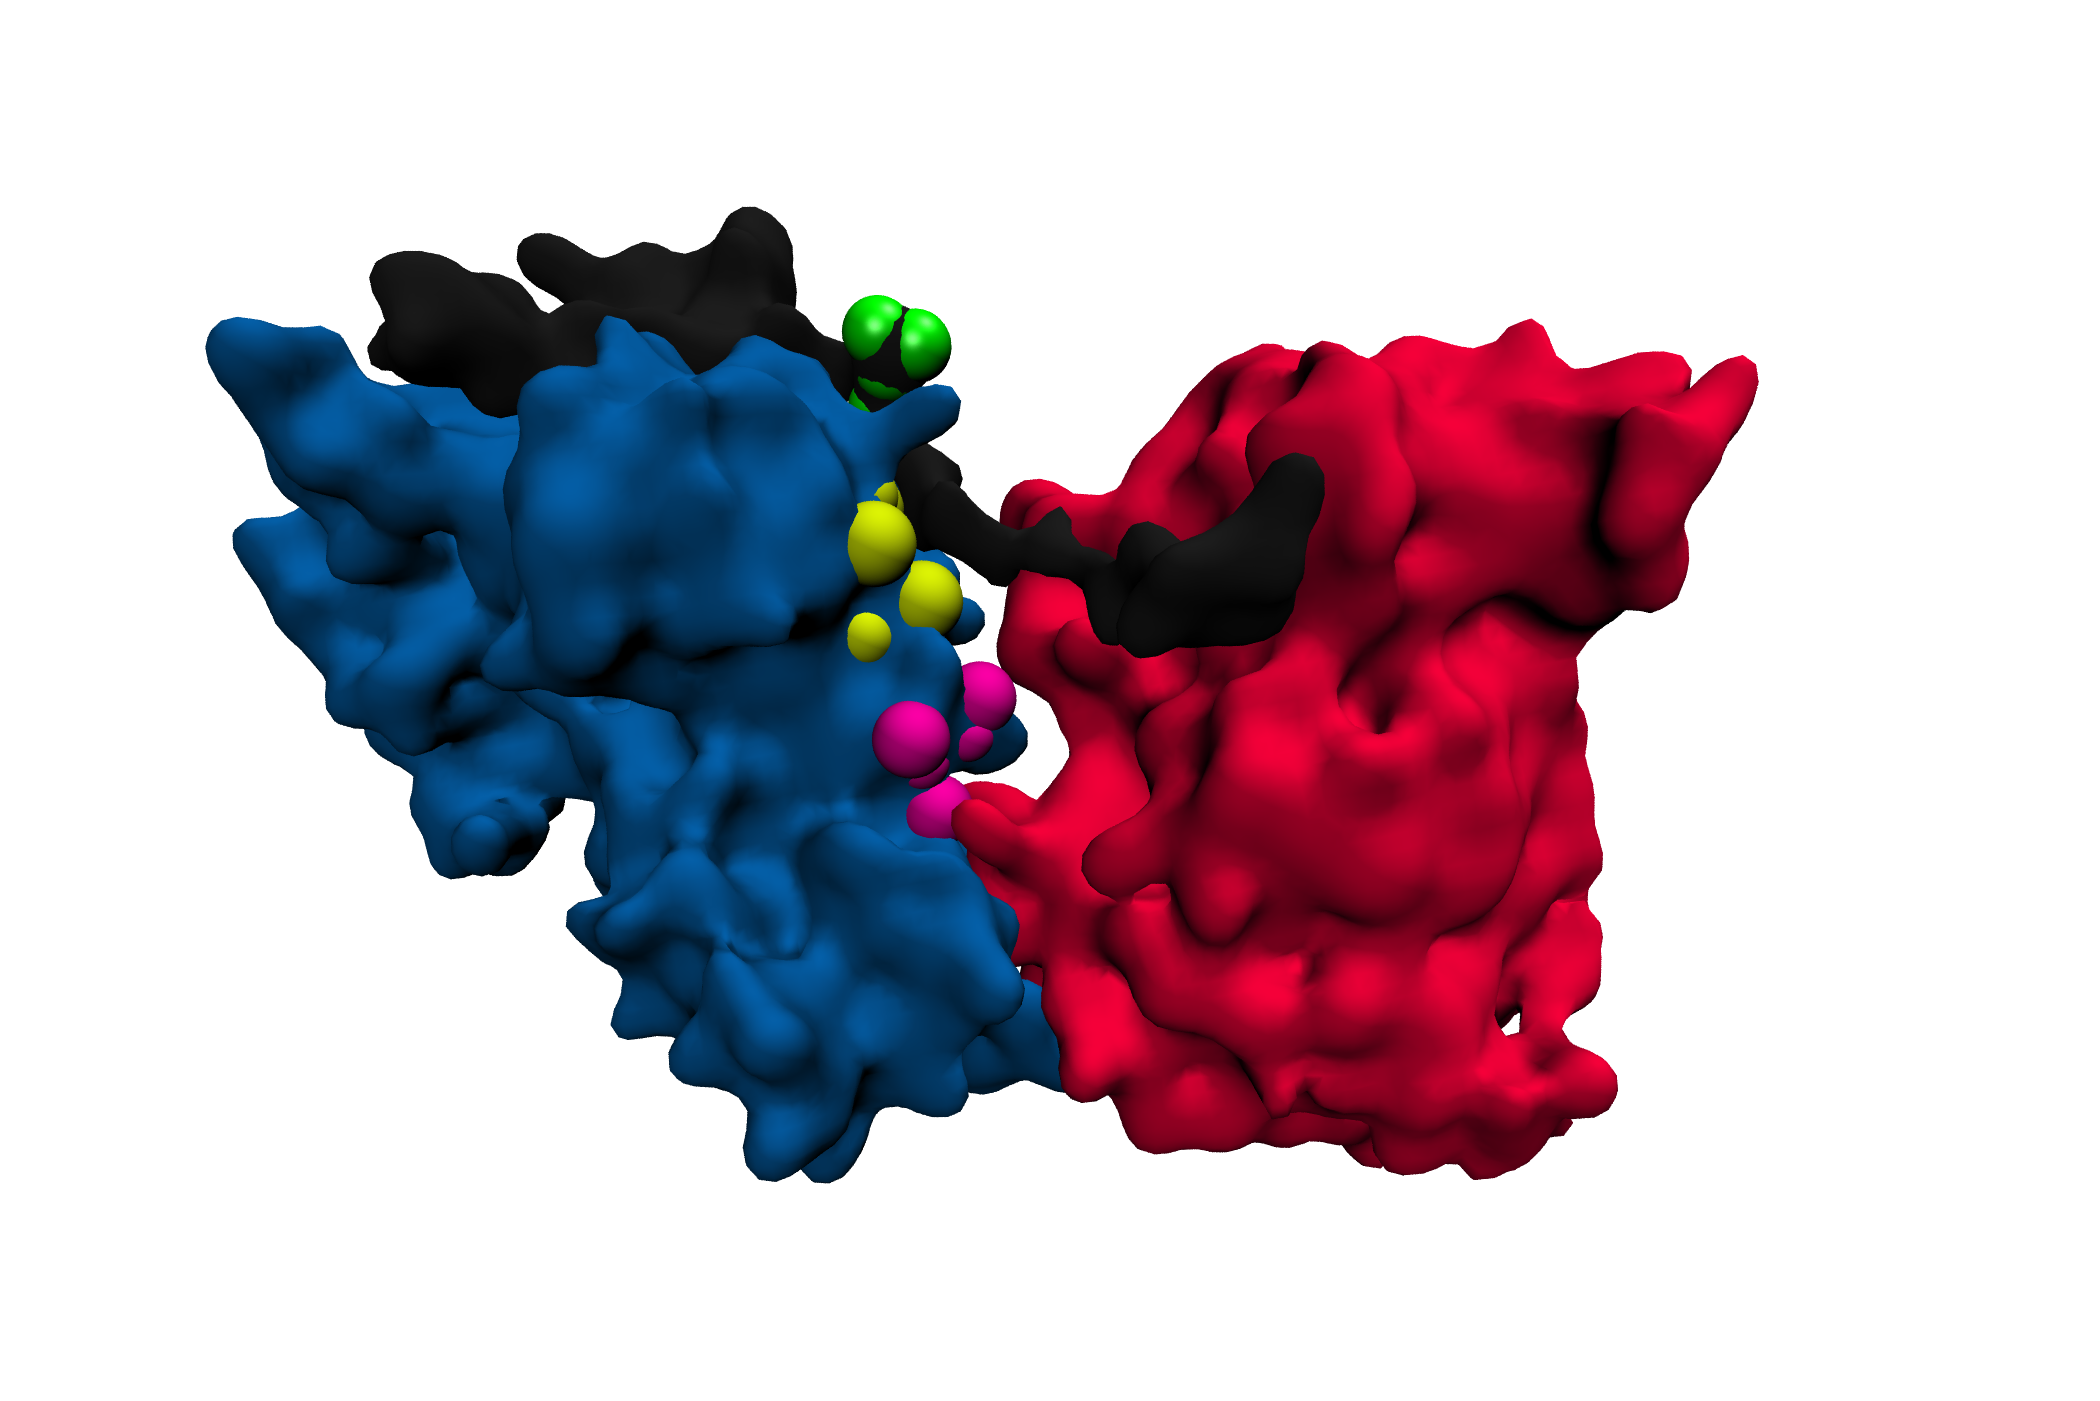
\includegraphics[height=4cm]{figures/results/fak_mem}
	\nicecaption{3D structure of FAK-MEM}{The 3D structure shows the FERM domain (blue), the kinase (red) and the linker (black, transparent). The molecule is located on the membrane (grey). The autophosphorylation site \acid{Y}{397} (green) is exposed. Residues around \acid{S}{47} (magenta) gets farther away from the kinase while residues around \acid{W}{52} (yellow) gets closer.}
	\label{mem:3d}
\end{figure}
%
%
%

%
%
\section{Multiple FAK interactions}
In this section the interactions occuring between multiple FAK molecules are analysed, for which the data from setup 4 is used. At this point the reader shall be reminded, that the used protein structure lacks the FAT domain, which is in full length FAK connected to the kinase via a linker region. This might make an important difference for clustering processes.\\
The characterisation of the emerged FAK clusters is very difficult as they differ a lot in size and shape. The largest cluster observed in setup 4 had a size of 21 proteins, while there are other proteins, which did not join any cluster at all. Present shapes of the clusters include long chains as well as ring like conformations or just an agglomeration (see \autoref{tobeadded}). Nevertheless in none FAK molecule the FERM domain dissociated from the kinase, which means no activation took place.\\
\\
For further analysis interactions between two proteins are classified into 9 different interaction types (see \autoref{einbildsagtmehralstausendworte}). Two proteins are interacting, if their minimal distance is smaller than $1.5\,\si{\nano\metre}$ and are called neighbours in this case. In contrast a protein belongs to a cluster, if it has at least one neighbour inside the cluster. A single protein without neighbours has clustersize 1.\\
First of all the mean number of neighbours is examined. One can see in \autoref{tobeadd} a fast rising in the number of neighbours in the beginning and a flattening after $6\,\si{\nano\second}$. The average of the five copies is at the end of the simulation $1.86$. This indicates a tendency to chains of FAK.\\
In \autoref{tobeadd} the average number of encounters of the different interaction types is plotted against the time. It shows, that FERM-kinase interactions (type 3) occur the most, while the others occur equally often. Only type 6 and type 7 (interactions, in which all four domains are involved) occur much less than the others.\\
From these observations one could draw the conclusion, that the preferred arrangement of FAK molecules is a chain, in which the FERM domain interacts with the kinase of the next molecule.


%In this section the interactions, which occur in FAK clusters, are analysed. At this point the reader shall be reminded of the limitation of our model, i.e. the dropping of the FAT domain. In contrast to our model full length FAK includes also a FAT domain which is connected to the kinase via a linker region. Therefore the observed interactions might be very different from those of full length FAK.\\
%The characterisation of the emerged FAK clusters is very difficult as they differ a lot in size and shape. The largest cluster observed in the five trajectories had a size of 21 proteins while there are other proteins, which did not join any cluster at all. Both, closed conformation like rings, as well as long chains were observed, as you can see f.e. in \autoref{tobeadded}.\\
%It is worth to analyse the neighbouring types in the cluster. In \autoref{tobeadded} the average number of neighbours for the five trajectories is plotted against the time. Although there are clusters of more than 20 proteins, the number of neighbours stays below 2 (maximum of the five trajectories is 2.5). \autoref{tobeadded} shows the number of encounters of a give neighbour type as a function of time. These, in which only two domains interact (FERM-FERM, FERM-kinase and kinase-kinase), occur most often, especially type 3 (FERM-kinase) appears very often. These findings may suggest, that chains of multiple FAK connected as type 3 neighbours are a preferred arrangement. However this could be a relict of dropping the FAT domain or too short simulation times since auto arrangement of large molecules like proteins is a slow process.\\
%Clustering of FAK did not induced activation in the simulations. At any time the minimal distance between the FERM domain and the kinase of one protein was lower than $0.8\,\si{\nano\metre}$ and also long ranged configurational changes could not be observed.
%
%
% chapter conclusion
\chapter{Conclusion}
The aim of the present work was to gain insight into conformational changes of FAK due to \pip{} binding and interactions between multiple FAK molecules. To this end, we used coarse-grained MD simulations with the \martini{} force field.\\
\\
Previous work in the group revealed unnatural behaviour of FAK bound to a \pip{}-containing membrane in \martini{} simulations, namely, a falling sidewards on the membrane. We were able to prove that this is not induced by an underestimation of \pip{} binding at the basic patch. Indeed, \martini{} was able to reproduce the free energy profile of this binding obtained from a reference simulation in \charmm{} remarkably well. However, the cause of the falling is still an outstanding question and should be addressed in further studies.\\ % FDA?
\\
In this project, we introduced a workaround, namely, a stabilising force acting on the FERM domain of the FAK molecules. In \autoref{forceana}, we showed that this approach does not influence the observables used in the remaining part, but we are aware of its limitations and still investigate possible alternatives, for example, flat-bottom pulling \autocite[p. 156-158]{gromacsManual}.\\
\\
From the configurations obtained for FAK in solution, we identified important residues contributing to the FERM-kinase interface. The observations fit well with experimental studies of \textcite{structFAK}. Also the burying of the active site of the kinase as well as the hiding of the autophosphorylation site were observed in the simulations.\\
We compared these results to conformations obtained in FAK molecules bound to a \pip{}-containing membrane and identified configurational changes. They involve not only the promotion of the autophosphorylation site, but also a partial opening of the FERM-kinase interface at the activation loop of the kinase. These changes are consistent with previous studies on allosteric effects of \pip{} binding to FAK by \textcite{pap001} and \textcite{pap003}.\\
\\
In \autoref{multiProt}, we investigated the interactions between multiple FAK molecules on a membrane. Our observations do not support a conclusion on the energetic preference of the different dimer types. Yet, we were able to confirm the importance of \acid{W}{266} in FERM-FERM dimerization proposed by \textcite{fakdimers}. Regarding more than two FAK molecules, we observed a tendency to aggregate in chain-like structures. These structures were investigated for activation-promoting features, like increased domain distances or a smaller contact area, but no significant differences have been observed.\\
\\
Several aspects of FAK clustering are still elusive and have to be clarified in further studies. First, the local aggregation and arrangement of FAK molecules is of special interest and could be investigated with further simulations of dimers, trimers and tetramers. With a deep understanding of these interactions, simulations of larger oligomers with a higher level of coarse graining could become accessible. Moreover, a more detailed analysis of the role of the membrane, especially the \pip{} concentration and membrane curvature, might contribute to the understanding of FAK clustering processes.



\end{document}